\documentclass[11pt]{article}
\usepackage[utf8]{inputenc}
\usepackage[T1]{fontenc}
\usepackage[margin=1.05in]{geometry}
\usepackage{amsmath,amssymb}
\usepackage{graphicx}
\usepackage{booktabs}
\usepackage{natbib}
\usepackage[expansion=false]{microtype}
\usepackage[font=small,labelfont=bf,skip=6pt]{caption}
\usepackage{authblk}
\usepackage{hyperref}
\hypersetup{colorlinks=true,linkcolor=black,citecolor=black,urlcolor=blue}
\usepackage{titlesec}
\titlespacing*{\section}{0pt}{12pt}{5pt}
\titlespacing*{\subsection}{0pt}{9pt}{3pt}
\setlength{\parskip}{4pt}
\renewcommand{\arraystretch}{1.05}
\bibliographystyle{apalike}

\title{\bfseries Robust Ensemble Forecasting in Practice:\\[2pt]
\large Model Selection and Combination Across Heterogeneous Time Series}

\author[1]{Anil Kumar Singh}
\author[1]{Sanvi Bhardwaj\thanks{Correspondence: \texttt{sanvi.b@lifesight.io}}}
\author[1]{Rajeev Aravindakshan Nair}
\affil[1]{Lifesight}
\date{}

\begin{document}
\maketitle

\begin{abstract}
\noindent Organisations forecasting large portfolios of heterogeneous series must decide whether to combine candidate models or choose among them. On 99 daily commercial series from 65 organisations, cut at three rolling origins into 293 out-of-fold cells with every selection and weighting decision made on a strictly prior validation window, a per-period trimmed mean matched the best single model available without having to identify it. Identifying it is the harder half: a portfolio-level rule restricted to evidence already available at the forecast origin trailed the ensemble by 0.13 mean RelMAE until roughly 150 cells had accumulated, then closed to 0.025. The ensemble sits at that level from the first cell, because it estimates no ranking. The two tie on typical accuracy and differ in what a bad quarter looks like: the single model lands in the worst three of eleven ranked methods in 17.4\% of cells against the ensemble's 1.0\%, a frequency statement about per-cell ranks rather than a claim about tail magnitude, which our intervals do not support. The ensemble carries the lowest mean and worst-case regret to the per-cell oracle of all twelve methods, beats every single model outright in 22\% of cells, and is never worse than third on any summary we report. Per-series selection is the floor of the same gradient, beaten in 200 of 293 cells (0.737 against 0.803; Holm-adjusted $p \approx 5.7\mathrm{e}{-9}$) and at the series and organisation levels, because within one cell validation error orders the five candidates with a mean rank correlation of 0.14 and picks the winner in 26\% of cells against 20\% for a blind draw. We recommend combination as the default, portfolio-level selection as a defensible alternative for mature panels, and per-series selection in no case. Evidence is a single corpus, so this is a candidate default rather than a settled one.

\vspace{6pt}
\noindent\textbf{Keywords:} forecast combination; ensemble forecasting; model selection; cross-series pooling; robust statistics; out-of-fold evaluation; demand forecasting; marketing-mix modeling; RelMAE.

\vspace{3pt}
\noindent\textbf{Code:} \url{https://github.com/lifesight/robust-ensemble-forecasting} (archived: \emph{[ZENODO DOI ON RELEASE]}).
\end{abstract}

\section{Introduction}

Every business of any size has to forecast not one series but many, and those series rarely resemble each other. Firms maintain heterogeneous daily series across products, regions, and business units, each with its own seasonality, promotional dynamics, covariate sensitivity, and noise profile. Two operational realities complicate the choice of method. First, the best-performing model differs from series to series; second, for any given series the best model can differ from period to period. Applying one model everywhere therefore appears to leave accuracy unrealised, while fitting and maintaining a bespoke model for each series introduces its own estimation risk, tuning burden, and operational fragility.

Combining forecasts is a classical and well-evidenced response. Since \citet{bates1969}, a large literature has established that combined forecasts frequently dominate their constituents \citep{clemen1989,timmermann2006,wang2023}. A striking and durable regularity, the forecast combination puzzle, is that simple combinations such as the equal-weighted mean are difficult to beat with estimated ``optimal'' weights, because the sampling error incurred in estimating weights typically exceeds the benefit of using them \citep{stock2004,smith2009}. A robust extension replaces the mean with trimmed or Winsorized means of the member forecasts, retaining the simplicity of averaging while limiting the influence of occasional wild members \citep{jose2008,kourentzes2019}.

A second literature answers the same problem from the other direction. Rather than abandoning selection, it makes selection estimable by learning across series: FFORMS selects a model per series from features using a classifier trained on a large reference corpus \citep{talagala2023}, and FFORMA learns combination weights the same way \citep{montero2020}, placing second in the M4 competition. \citet{kourentzes2019} compare selection, combination and pooling directly and find that pooling information across series improves both. The common premise is that the per-series decision fails for want of data, and that data can be borrowed from elsewhere in the portfolio.

That premise is usually asserted rather than measured, and it is measured here. We hold the information set, the candidate panel and the evaluation protocol fixed, and vary only the quantity of evidence standing behind each selection decision. At one extreme a rule chooses per series from a single short validation window. At the other it chooses once for the whole portfolio from every validation window in it. Between the two sits a rule restricted to the evidence already available when the forecast is issued, whose pool accumulates over time. Comparing these against a robust combination that estimates no ranking at all turns a binary question --- combine or choose --- into a measurable gradient.

The gradient is steep at the bottom and flat at the top. Per-series selection is beaten decisively and at every unit of aggregation. Portfolio-level selection improves rapidly as evidence accumulates and reaches parity with the ensemble --- but has to accumulate the evidence first, whereas the combination is at that level throughout, having no ranking to estimate. The mechanism is visible directly in the selection signal: within a cell, validation error ranks the five candidates with a mean rank correlation of 0.14 against their eventual test ranking. This is not an artefact of scoring the two sides with different losses, since the matched-loss figure is the one we quote, and not an artefact of low daily counts, which we test by splitting the corpus at the median.

We make five contributions. First, a large out-of-fold benchmark quantifying how often each single model is best and how four combination rules compare on typical accuracy, tail risk and regret, with formal significance testing, effect sizes, and a standard Theta benchmark. Second, we isolate decision granularity as the operative variable by holding information and candidate set fixed across three selection strategies that differ in nothing else. Third, we show that the crudest conceivable pooled rule --- one model for the entire portfolio, no features, no meta-learner --- recovers essentially all of the distance between per-series selection and a robust ensemble, which bounds from below what pooling is worth and from above the incremental credit that the feature-based methods of \citet{montero2020} and \citet{talagala2023} can claim on a panel like this one. Fourth, we introduce a family de-duplication construction treating models that share a methodology as one family, and report an ablation establishing what it does and does not buy. Fifth, we apply a uniform inferential standard: every tail statistic and subgroup comparison carries a series-clustered bootstrap interval, every comparison in the primary family carries an effect size and a multiplicity correction, and every headline comparison is repeated at the cell, series and organisation levels.

\section{Related work}

\subsection{Forecast combination}

Forecast combination originates with \citet{bates1969}, who showed that a weighted combination of two forecasts can attain lower error than either constituent, with weights derived from past error variances. \citet{clemen1989} surveyed the subsequent two decades and distilled a consensus that has since held: combination robustly improves accuracy, and simple schemes often rival or beat complex ones. \citet{timmermann2006} provides the standard theoretical account, including the conditions under which equal weighting is optimal or near-optimal. \citet{wang2023} survey the fifty years since Bates and Granger and document that the basic finding has survived every subsequent methodological wave, and \citet{petropoulos2022} give a broad treatment of current practice covering combination, selection and pooling together.

The forecast combination puzzle, that the equal-weighted average routinely outperforms estimated optimal weights out-of-sample, was documented by \citet{stock2004} and given a clear finite-sample explanation by \citet{smith2009}: estimating weights injects variance that generally dominates the bias it removes, especially when members are numerous or of similar quality. Within that tradition, \citet{jose2008} study trimmed and Winsorized means and report that they slightly improve on the mean while reducing the incidence of large errors, with the advantage greatest when the individual forecasts are highly variable; \citet{kourentzes2019} reach a similar conclusion for the median as a combination operator. Our reading of the present results places per-series model selection on the same continuum: it is the limiting case of estimated weighting, in which all the weight is placed on the validation winner, and it fails for the same finite-sample reason, only more so.

The empirical scale of the effect is established by the M competitions. \citet{makridakis2020} report that combinations occupied most of the leading positions in M4, and \citet{makridakis2022} that machine-learning methods, gradient boosting in particular, dominated M5's retail hierarchies. Our finding that CatBoost is the strongest single member on a daily retail panel is a replication of the second of those results rather than a novel observation, and we treat it as such.

\subsection{Selection, and pooling information across series}

\citet{fildes2015} compare simple and complex selection rules and find that the advantage of individual selection is easily destroyed by estimation error. \citet{petropoulos2018} decompose the sources of that error and show that model uncertainty, rather than the choice of candidate set, is what limits per-series selection. Both point at the diagnosis we reach here.

The most direct response is to stop estimating the selection rule one series at a time. FFORMS \citep{talagala2023} trains a classifier on features of a large reference set to predict which model will win on a new series; FFORMA \citep{montero2020} replaces the hard choice with learned combination weights; \citet{kourentzes2019} pool forecasts and information across series without a meta-learner. In all three the operative move is the same: borrow evidence from other series so that the per-series decision need not be estimated from the per-series data alone.

Our contribution sits underneath that literature rather than alongside it. Those methods condition the pooled decision on series features and require a meta-learner trained on a reference corpus. We ask what the pooling alone is worth, by stripping the construction to its crudest form: one model applied to the entire portfolio, chosen on aggregate validation error, with no features and nothing learned. If that crude rule already matches a robust ensemble, the incremental credit due to feature conditioning is correspondingly bounded, and a practitioner without the infrastructure for a meta-learner is not excluded from the benefit. We also measure how much pooled evidence the crude rule needs before it works, which the feature-based literature does not report.

\subsection{Evaluation, comparison, and base learners}

\citet{hyndman2006} introduced the mean absolute scaled error (MASE) and in the same paper catalogued the relative-error measures of which our headline metric is one; they also give the standard warning about averaging ratios across series, which motivates our reporting of the geometric mean alongside the arithmetic mean. For comparing many methods across many datasets, \citet{demsar2006} recommends the Friedman rank test with Nemenyi post-hoc analysis, which we follow. For direct pairwise comparisons we draw on the \citet{diebold1995} tradition, adapted to a Wilcoxon signed-rank test since our panel is many short heterogeneous series rather than one long series. \citet{assimakopoulos2000} introduced the Theta method, our canonical simple benchmark. \citet{kolassa2016} sets out why percentage-based measures behave badly on low-count retail demand, which bears on our choice of validation criterion (Section~\ref{sec:rules}).

Our panel spans deliberately dissimilar methodologies so that member errors are imperfectly correlated: SARIMAX, a classical seasonal ARIMA with exogenous regressors \citep{seabold2010}; a Bayesian structural time-series model in PyMC \citep{salvatier2016,abrilpla2023}; the additive-decomposition models Prophet \citep{taylor2018} and NeuralProphet \citep{triebe2021}; and gradient-boosted decision trees via CatBoost \citep{prokhorenkova2018}. Our contribution is not a new base learner but a large-scale evaluation of combination and selection over such a panel.

\section{Data}

\subsection{Corpus}

We evaluate 99 daily commercial time series belonging to 65 organisations. Each series is an organisation--territory pair, and the forecasting target is daily total purchases. The corpus is deliberately heterogeneous: the point is to test methods across series that differ in seasonality, scale, and noise, rather than across variants of one well-behaved series. In the source taxonomy, 91 of the 99 series fall into 13 named industry verticals and the remaining 8 are unclassified; the 91 divide into 30 named subverticals.

The series are drawn from a publicly available e-commerce marketing dataset \emph{[SOURCE DATASET CITATION TO BE INSERTED]}. We did not collect or commission the data and claim no ownership of it; our contribution at this stage is the qualification screen described in Section~\ref{sec:cleaning}, which selects the 99 series meeting a strict history-length, completeness and coverage bar from a larger candidate pool. Because the underlying data are public, the corpus, the screen, and everything derived from them can be inspected and re-derived by anyone.

Each series carries three exogenous covariates capturing daily paid-media spend, aggregated to Google, Meta, and TikTok totals by summing the per-channel spend columns of the source data. These covariates are decision variables known in advance at forecast time, since media plans are set ahead, so using their contemporaneous values introduces no look-ahead bias.

\subsection{Cleaning and qualification}
\label{sec:cleaning}

Series were keyed on the organisation--territory identifier, which dissolved apparent duplicate rows arising from multiple territories per organisation, and per-channel spend was aggregated to the three covariate totals, treating missing channel entries as zero spend. One organisation exhibiting a corrupt single-day spike more than three orders of magnitude above its median was removed as a data-quality failure before qualification; this removal preceded the candidate manifest and is therefore not recorded in it.

Series were retained only if they met a strict quality bar: at least 600 days of history, to support a three-way temporal split with rolling origins; no calendar gaps; no zero-target days, which would destabilise percentage errors; and paid-media spend present on at least 90\% of days. Of 142 candidate series, 99 qualified. Of the 43 excluded, 33 failed on history length alone, 6 on media-spend coverage alone, and 4 on both; no candidate reaching this stage failed on calendar gaps or zero-target days, so those two screens never bind in the deposited manifest. An exclusion rate of 30\% is material to generalisation, and we return to it in Section~\ref{sec:caveats}. The resulting corpus spans 611 to 1,751 days per series (median 1,030) over July 2019 to June 2024, totalling 106,924 daily observations.

Two structural features bear on interpretation. First, many series carry low daily counts: mean daily purchases per series range from 9.2 to 688 (median 49.7), with 18 of the 99 series averaging fewer than 20 per day and 50 fewer than 50. These figures are not a comparison of business size, since organisations differ in what they sell and at what price and basket size. We report the distribution because the lower a series' daily count, the larger the share of its variance that is Poisson-like arrival noise rather than predictable structure, and that noise floor caps how far any method can improve on the benchmark. It is the most likely explanation for the 13\% of cells in which the reference ensemble fails to beat seasonal-naive and the 10 cells (3.4\%) in which no method beats it at all. It also bears on the validation criterion, since percentage-based losses are least reliable exactly where counts are lowest \citep{kolassa2016}; Section~\ref{sec:granularity} tests whether that drives our central result and finds it does not. Comparability across organisations is handled by the metric rather than the counts: every figure we report is a ratio of each series' error to its own benchmark error, and no raw purchase count is ever pooled across series.

Second, the 99 series correspond to 65 distinct organisations. Eleven contribute more than one territory series, and the largest contributes ten. Because a territory of one organisation sells a different product mix into a different market, we treat series as the natural independent unit, but rest no conclusion on that choice and report organisation-clustered versions of every headline test in Section~\ref{sec:units}. The territory field is not carried in the deposited dataset, which records only the hashed series and organisation identifiers.

\subsection{Data and code availability}

The qualified corpus is released in full alongside this paper, together with the per-cell base-model forecasts, the per-cell summary metrics including validation as well as test losses, the split boundaries for every cell, and the scripts that generate every number and figure below. Details are in the Statements section before the references.

Every quantity reported here can be regenerated from the deposited artefacts without refitting any model. What cannot be regenerated is the forecasts themselves: base-model fitting code is released as part of the Horizon forecasting library (Section~\ref{sec:conclusion}) rather than in the analysis repository, so a reader working only from the deposited artefacts can reproduce every table and figure but must go to the library to re-derive the inputs. The deposited dataset is the qualified corpus rather than the public source, so Sections 3.1--3.2 can be confirmed against it directly and reproduced from the public source using the deposited screen; the candidate manifest records the disposition of all 142 candidate series, which is what makes qualification auditable.

\section{Methodology}

\subsection{Out-of-fold, rolling-origin evaluation}
\label{sec:design}

Each series is partitioned chronologically into three contiguous blocks: a training window used to fit the base models, a validation window used solely to select and weight models, and a held-out test window used solely for reporting. The ordering is always train, validation, test in time, so every selection decision precedes the reported window, mirroring deployment. Validation and test windows are each 12\% of series length. We repeat at three successive origins per series, stepping the windows back by one test-block each. Training therefore grows from roughly 52\% of the series at the earliest origin to 76\% at the latest, and the three test windows of a series are disjoint. This yields 297 candidate cells ($99 \times 3$), of which 293 have complete forecasts from all five base models. The four dropped cells are those in which a base model failed to fit or converge, three involving NeuralProphet and one SARIMAX; we drop the whole cell rather than evaluate the remaining methods on it, so every method is scored on an identical set.

That decision has a consequence worth naming. Every figure here is conditional on all five base models converging, which flatters the strategies requiring the full panel --- the four combinations and per-series selection --- relative to a deployment in which a member can fail. Portfolio-level selection is the one strategy not exposed to this. At 4 cells in 297 the magnitude is negligible; the asymmetry is the point.

The benchmark and the models are not issued from the same origin. The models forecast from the end of training, while the seasonal-naive benchmark is built from the last week before the end of validation (Section~\ref{sec:models}), so the benchmark sees one validation block the models do not. Reported RelMAE values are therefore conservative, understating the models' advantage over a benchmark issued from their own origin. Because the same benchmark divides every method within a cell, no comparison among methods is affected. It does mean the effective lead time exceeds the quoted test-window lengths, roughly by a factor of two.

With that recorded, the evaluation is a long-range one. Each cell requires a single multi-step forecast issued from the origin and never revised. Test windows run from 73 to 210 days (quartiles 96 and 158, median 123, mean 129), and the lead time to the far end is roughly twice that. This is the planning horizon these businesses work to, but far longer than the one- to seven-step evaluations that dominate the combination literature, and it is one reason the seasonal-naive benchmark is beatable by wide margins here.

\subsection{Base models, benchmark, and admissibility}
\label{sec:models}

Five base models are fit per cell: SARIMAX, a Bayesian structural model (PyMC), Prophet, NeuralProphet, and CatBoost. Each emits a point forecast over the test horizon. SARIMAX, CatBoost, Prophet and NeuralProphet consume the three known-in-advance media-spend covariates as regressors; the Bayesian structural model consumes them as a regression component; Theta, a competitor rather than a member, uses none. Every model is configured by the same procedure --- a common grid search scored on validation error, applied identically in every cell --- so no model receives tuning attention the others do not; the search spaces, seeds and library versions are recorded with the released fitting code.

A seasonal-naive forecast serves as the benchmark, and its construction matters, because the alternative would invalidate every RelMAE number in the paper. The benchmark repeats a single fixed week across the entire test window, so that a test day $t$ is predicted by the same weekday of that one week. It is \emph{not} a rolling lag-7 of test actuals, which would let the benchmark consume realised outcomes the models never see. The week used is the last one observed before the end of validation.

The target is a strictly positive count, so a negative point forecast is not admissible. We impose $\hat{y} \leftarrow \max(\hat{y}, 0)$ on every member before any evaluation or combination. This is a specification correction rather than a tuning choice, applied uniformly to all five base models and to Theta. In practice it binds on Prophet alone, and rarely even there: 837 of 189,420 member-observations are affected, all of them Prophet's. For Prophet the constraint improves mean RelMAE from 1.114 to 0.960, while the remaining four members and the trimmed ensemble are numerically unchanged.

\subsection{Family de-duplication}
\label{sec:dedup}

Prophet and NeuralProphet share the same additive-decomposition methodology (trend plus seasonality plus regressors), so an ensemble containing both effectively places two votes on that single hypothesis. We de-duplicate the family as the core construction: within each cell we retain only the member with the lower validation MAPE among \{Prophet, NeuralProphet\}, yielding a four-member set $M$ = \{chosen additive-decomposition model, CatBoost, SARIMAX, Bayesian\}. All combinations operate on $M$. The rationale is structural rather than empirical: two instantiations of one methodology are not two independent views of the data. Resolving the family per cell rather than globally is warranted by the split itself, Prophet being the representative in 60\% of cells and NeuralProphet in 40\%. Section~\ref{sec:ablation} reports the ablation.

The two are not identical implementations: NeuralProphet admits autoregressive components that Prophet does not, so treating them as one family is a claim that needs support rather than assertion. The support is empirical. Across all test observations the signed-error correlation between Prophet and NeuralProphet is 0.787, the highest of any pair in the panel involving either model and well above their correlations with CatBoost (0.646 and 0.687) or with SARIMAX (0.493 and 0.458); the panel mean is 0.63 (Section~\ref{sec:diversity}). Whatever the architectural difference contributes, these two members make the most similar errors of any pair here, which is the property de-duplication exists to address. We therefore motivate the family structurally and verify it empirically, rather than relying on either alone.

\subsection{Combination rules and the three selection baselines}
\label{sec:rules}

Let the four members produce forecasts $f_1(t), \dots, f_4(t)$ for test period $t$, with validation errors $e_1, \dots, e_4$ (validation MAPE). We evaluate four combination rules.

\textbf{Trimmed mean (reference).} For each $t$, discard the highest and lowest member forecasts and average the remainder. With four members this averages the middle two, which is the per-period median; we therefore describe the rule as a per-period median throughout, retaining the trimmed-mean framing only where generalisation to larger panels is at issue. Every empirical claim made for it here is a claim about the median of four members.

It is worth naming what this rule does, because the framing of combination as the opposite of selection obscures it. Discarding the extreme members each period \emph{is} a selection decision: it excludes whichever members are furthest from the consensus on this series in this period. What distinguishes it from the selection baselines below is not that it declines to choose but that it chooses at a different granularity and estimates nothing to do so --- the decision is taken per period from the members' own disagreement, with no validation ranking, no weights, and no parameters. Section~\ref{sec:diversity} shows this is not a formality: within a cell the excluded member is highly persistent, so trimming behaves in practice like an automatic, per-cell exclusion of a systematically misbehaving member, arrived at without anyone having to identify it.

\textbf{Mean.} The equal-weighted average, $\tfrac{1}{4}\sum_j f_j(t)$.

\textbf{Weighted.} A weighted average with $w_j \propto 1/e_j$, normalised so $\sum_j w_j = 1$.

\textbf{Screened ($\geq 2$).} An equal-weighted average over members whose validation MAPE falls below $\tau = 0.40$, requiring at least two qualifiers; otherwise it falls back to the equal mean of all members, which triggered in 13\% of cells.

The four rules trace a progression: an estimation-free robust centre, the classical simple average, an estimated-weight scheme the combination puzzle predicts should struggle, and a scheme conditioning membership on validation performance. Every rule is applied in identical form to all 293 cells. None is tuned per series, vertical, or origin; none is given a fallback activating on inspection of results; and no rule sees any test-window quantity at any point.

The recommended rule has no free parameter. Two constants appear among the comparison rules. The trim depth is one member from each end, the minimum non-degenerate trim and the only depth available at four members, so it is fixed by construction. The screening threshold $\tau = 0.40$ was set as a competence floor, on the reasoning that a validation MAPE of 40\% on a daily series is poor by any standard; it was fixed before any test-window result was computed and never revisited. We note this is an assertion about our own process rather than a preregistration, and it should be weighed as such. Rather than rest on it, we report what the choice is worth (Table~\ref{tab:tau}). Sweeping $\tau$ from 0.20 to 0.80 moves the screened rule's mean RelMAE by 0.018 in total, from 0.747 to 0.764, with no monotone trend, while the fallback rate --- the share of cells in which fewer than two members qualify and the rule reverts to the equal mean --- falls from 67\% to 1\%. The screened rule trails the trimmed mean at every value of $\tau$ we tried. The threshold is therefore not a consequential parameter: no setting of it changes which rule we recommend, and the rule it governs is not that one.
We then add three non-combining strategies, all supplied with the same fitted models and the same absence of any test-window quantity. They differ in how much validation evidence stands behind each decision, and that controlled difference is the paper's central object of study.

\textbf{Per-series validation-selected model.} Within each cell, take the base model with the lowest validation MAPE among all five and use its forecast alone. This is the ex-ante analogue of per-series selection as practised. Restricting the same rule to the four de-duplicated members returns an identical model in every cell, so the comparison against the ensemble is not an artefact of the ensemble having been de-duplicated while the selector was not.

\textbf{Accumulating portfolio-selected model.} At each cell, rank the five models by validation MAPE aggregated over every cell whose validation window had already finished when this cell's forecast was issued, and apply the winner. The evidence available grows over calendar time, and Section~\ref{sec:pooling} uses this to trace how quickly portfolio selection becomes reliable.

\textbf{Full-panel portfolio-selected model.} Rank the five models by validation MAPE aggregated across the whole portfolio at once, take the winner, and apply it to every cell. On this corpus the winner is CatBoost (mean validation MAPE 0.285 against 0.303 for the next-best SARIMAX), and it wins at all three rolling origins on both the mean and the median. Because it resolves to CatBoost's forecast path here, the CatBoost row of every table does double duty as the full-panel selection row.

None of the three should be confused with the per-cell oracle, which picks the best model using test-set outcomes and is reported only as an unattainable reference for the regret column. Theta is evaluated as an additional method and deliberately held outside the member set, so that every ensemble figure is pre-specified independently of it.

One feature of the selection comparators needs addressing, and the design settles it directly. The selection rules rank candidates by validation MAPE, and the inverse-error weights and screening threshold use the same quantity, whereas methods are scored on MAE-based RelMAE, so criterion and evaluation metric are not the same loss. Because test MAPE is retained per cell, the matched-loss comparison is available without additional fitting. Ranking members by validation MAPE against their eventual test MAPE --- the same loss on both sides --- orders the five models with a mean within-cell rank correlation (Spearman) of 0.14 and picks the eventual best model in 26.0\% of cells. The mismatched comparison gives 0.10 and 21.8\%. We report the matched pair throughout, as the more conservative of the two. Scoring per-series selection on that same loss does not change the ordering either (mean test MAPE 0.346, against 0.331 for full-panel selection and 0.318 for the trimmed ensemble).

A related objection is that validation MAPE is simply a poor criterion where many series carry low daily counts \citep{kolassa2016}. The matched-loss check does not address this, since it holds the criterion fixed and varies only the evaluation loss. Section~\ref{sec:granularity} addresses it directly by splitting the corpus at the median daily count. A fully decisive answer would re-run selection on a validation MAE criterion, which requires validation-window forecasts rather than validation-window summary losses; those are not retained by the current pipeline, and their retention is the first item of future work.

\subsection{Metrics}
\label{sec:metrics}

For a method producing forecast $\hat{y}$ over a test window with actuals $y$, we report the relative mean absolute error against the seasonal-naive benchmark,
\[
\mathrm{RelMAE} = \mathrm{MAE}(y, \hat{y}) \,/\, \mathrm{MAE}(y, \hat{y}_{\text{naive}}),
\]
where values below 1 beat the benchmark and lower is better. Because the naive scale cancels, RelMAE is scale-free and equals the ratio of the two methods' MASE values \citep{hyndman2006}, permitting aggregation across organisations of very different magnitude. It is a relative-error measure, not itself a scaled error. Per method we summarise the mean, geometric mean, median, 90th, 95th and 99th percentiles and the maximum, the fraction of cells beating the naive benchmark, and the regret to the per-cell oracle,
\[
\mathrm{regret}_i = \mathrm{RelMAE}_i - \min_j \mathrm{RelMAE}(\text{base model } j)_i ,
\]
which is how far a method sits above the best of the five base models chosen in hindsight for that cell; Theta is not in the minimand. Regret is the metric that answers the question a practitioner actually faces, and it is worth stating its operational reading. It is what you pay for having guessed wrong about which model would win: mean regret is the expected cost of that uncertainty, and maximum regret is the worst that uncertainty ever cost on this panel. A single model's regret is the price of a bet; a combination's is the price of declining to bet. Regret can be negative, since a combination may beat every one of its members on a cell. Because per-cell values within a series are dependent, all confidence intervals, on means and tail quantiles alike, come from a nonparametric bootstrap resampling series rather than cells.

We report the geometric mean alongside the arithmetic mean, with a bootstrap interval on each. RelMAE is a ratio, and the arithmetic mean of ratios is upward-biased and disproportionately sensitive to cells where the naive benchmark is strong and the denominator small, which is the objection \citet{hyndman2006} raise. The geometric mean is the appropriate central tendency for a ratio and is the number we would defend if the two disagreed; in this corpus they do not disagree on the ordering of the leading group or the identity of the best method, and headline pairwise tests are reported on both raw and log differences.

\subsection{Statistical comparison}
\label{sec:stats}

Following \citet{demsar2006}, we test for overall differences with the Friedman test on per-cell ranks and, where it rejects, identify statistically indistinguishable groups with the Nemenyi critical-difference (CD) procedure at the 0.05 level, $\mathrm{CD} = q_\alpha \sqrt{k(k+1)/6N}$. Here $k = 11$ --- five single models, Theta, per-series selection, and four combinations --- over $N = 293$ cells. Full-panel portfolio selection is excluded from the rank analysis, since on this corpus it resolves to an existing column and entering the same forecast path twice would inflate $k$; its verdict is read off the CatBoost row. The accumulating portfolio rule is a distinct path and is compared separately in Section~\ref{sec:pooling}.

We additionally run direct pairwise comparisons between the reference ensemble and each of its ten competitors using Wilcoxon signed-rank tests on cell-level RelMAE differences, in the spirit of \citet{diebold1995}. The Wilcoxon test assumes differences are symmetrically distributed under the null, which ratios satisfy only approximately, so we report a sign test alongside it for the two headline comparisons. Three further disciplines are imposed. \emph{Multiplicity:} we report Holm-adjusted $p$-values across the primary family of ten. Analyses outside that family --- the tail comparisons of Section~\ref{sec:tails}, the ablation of Section~\ref{sec:ablation}, the unit checks of Section~\ref{sec:units}, the per-vertical intervals of Section~\ref{sec:verticals} and the pooling analysis of Section~\ref{sec:pooling} --- are not part of the correction and should be read as supporting or exploratory rather than confirmatory. \emph{Effect size:} every $p$-value is accompanied by the rank-biserial correlation and the mean difference, because at $N = 293$ a Wilcoxon test will detect differences far too small to act on. \emph{Unit of analysis:} the 293 cells are not independent, so we repeat every headline test at the 99 series and the 65 organisations, averaging within the unit first. A result holding at all three units is reported as robust; one that does not is reported as not robust rather than at whichever unit is most favourable.

\section{Results}

\subsection{No single model dominates}

Across the 293 cells the identity of the best single model rotates: CatBoost is best in 34\% of cells, the Bayesian model in 20\%, Prophet in 18\%, NeuralProphet in 16\%, and SARIMAX in 11\% (Figure~\ref{fig:rotation}). No model is best in more than a third of cases. This is the empirical premise for combination, and the observation that has historically motivated per-series selection. Section~\ref{sec:granularity} shows the premise supports the first conclusion but not the second: rotation establishes that no fixed model is always right, not that the rotation is predictable in advance. Section~\ref{sec:diversity} gives the evidence that it reflects genuinely different failure modes, in the form of member error correlations well below one.

\begin{figure}[htbp]\centering
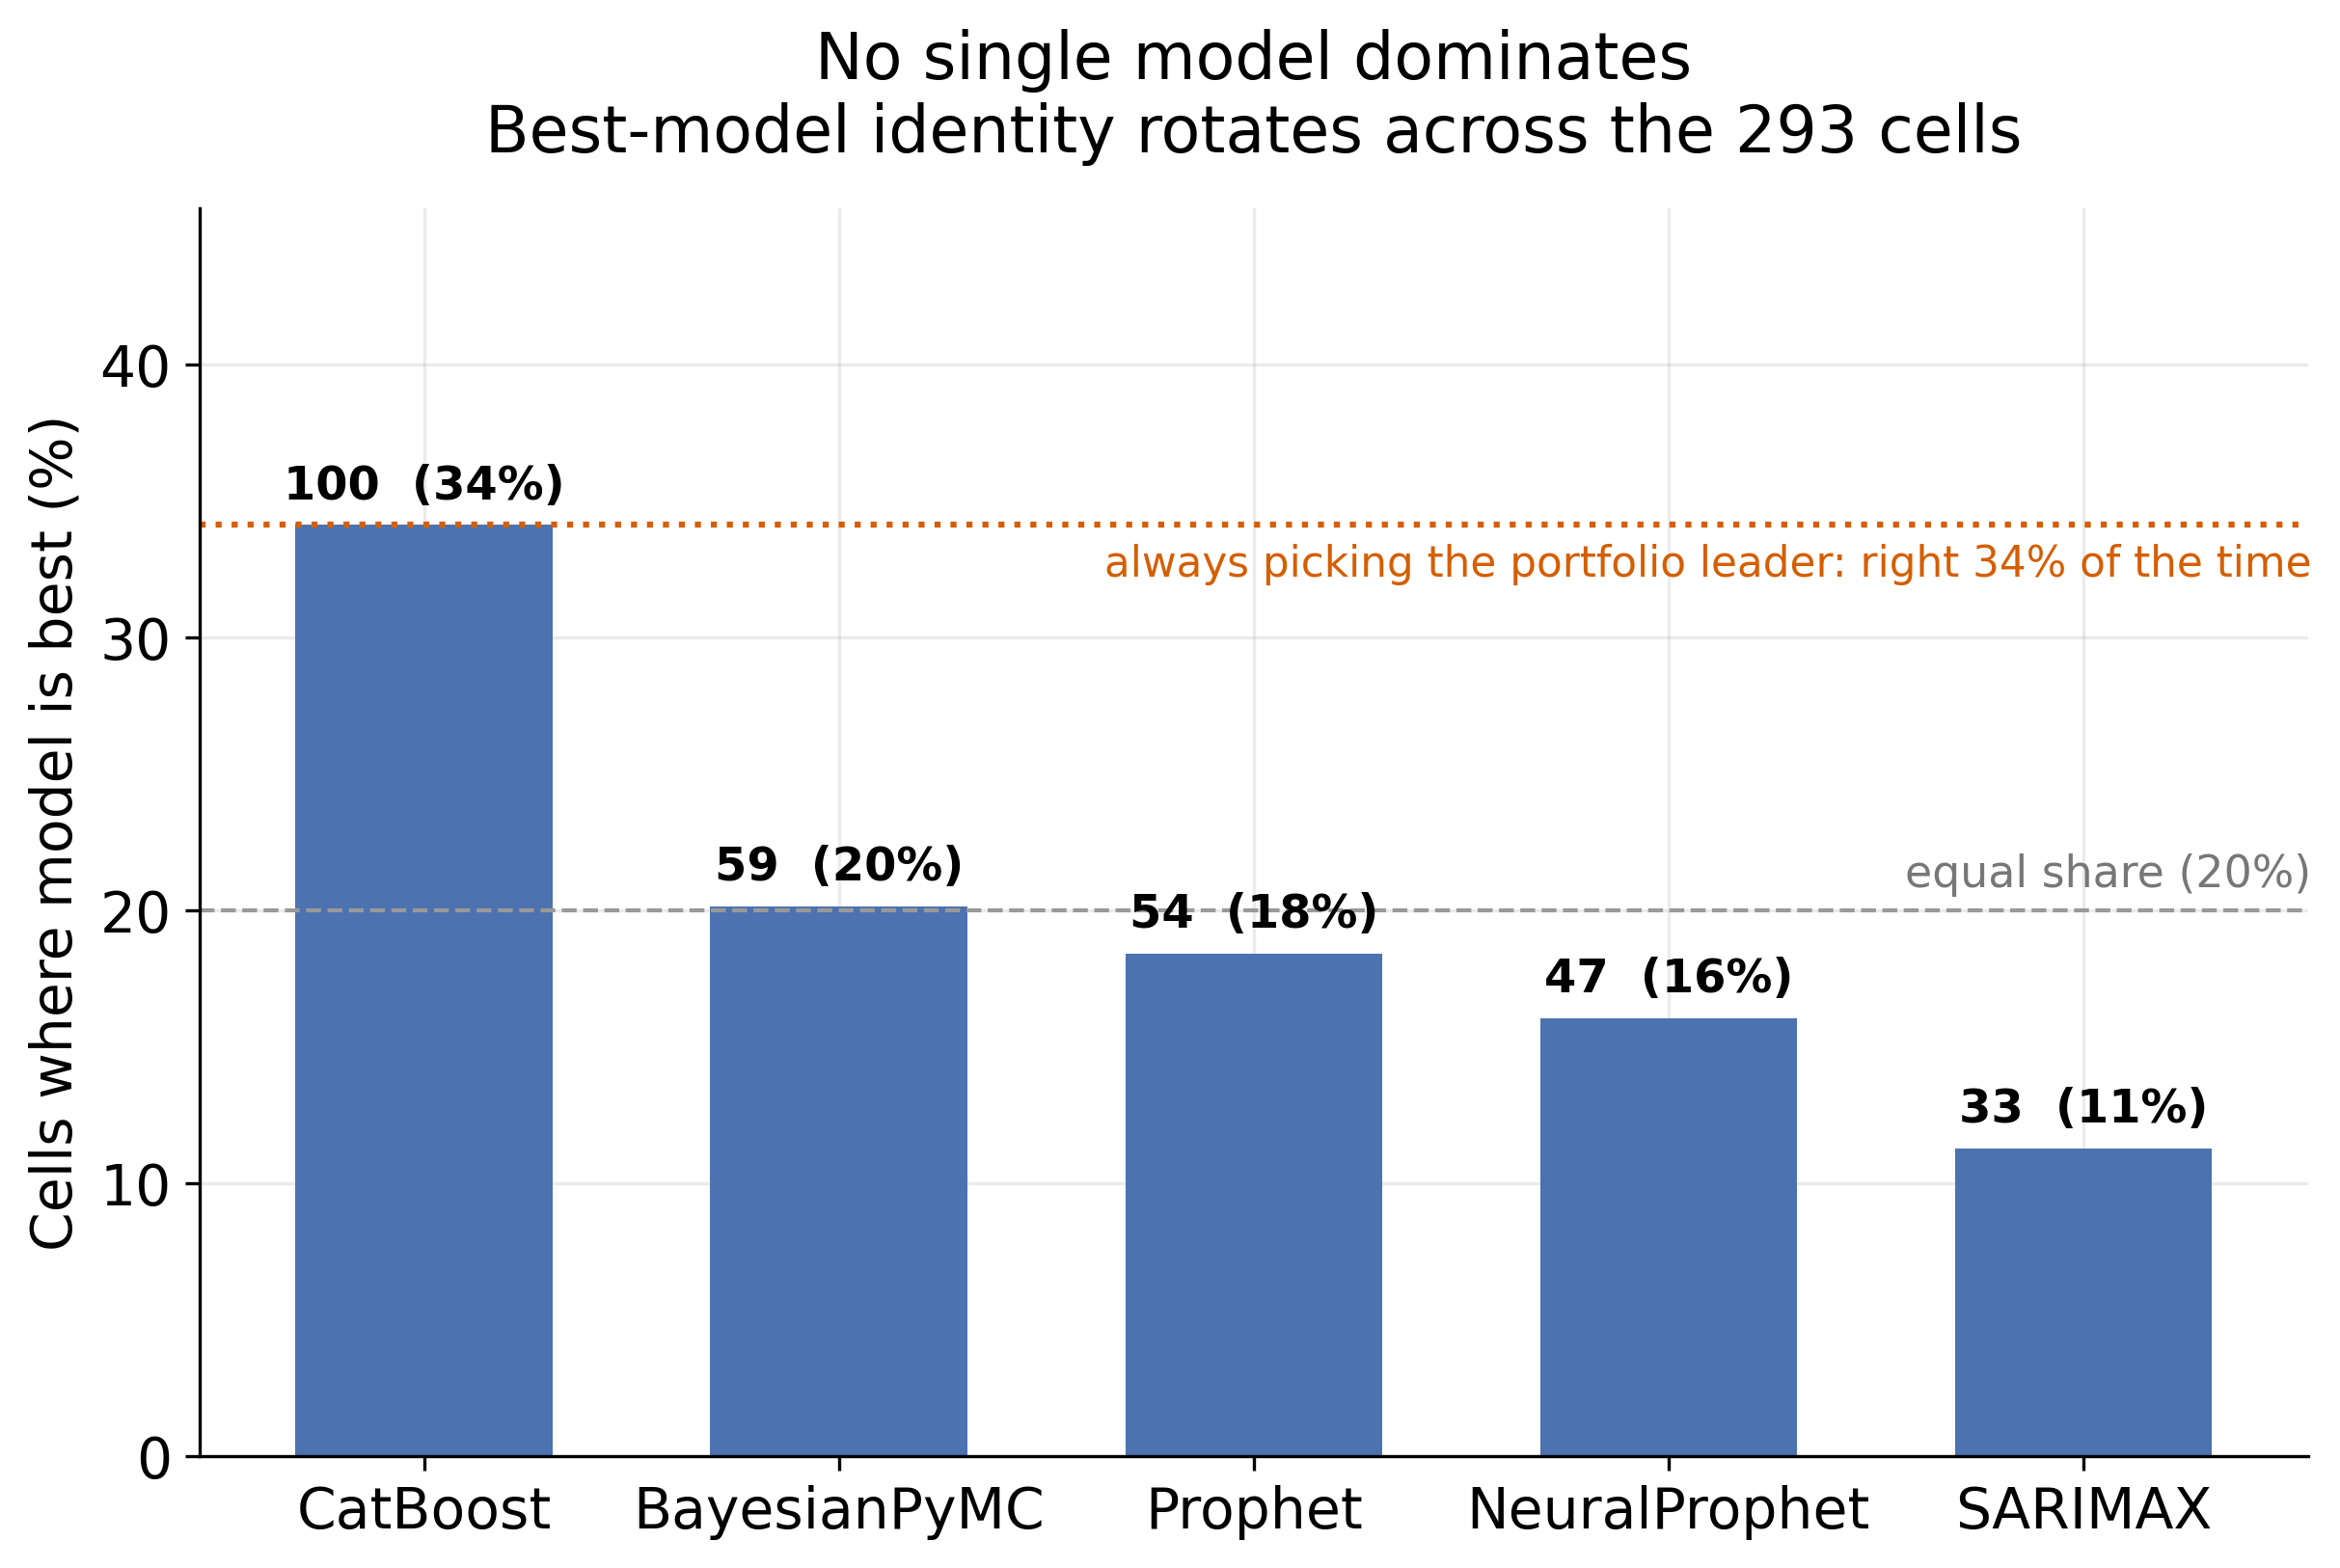
\includegraphics[width=0.86\textwidth]{../figures/figure01.png}
\caption{Share of out-of-fold cells on which each single model attains the lowest error. The dotted line marks how often the portfolio leader is best, the accuracy a constant rule achieves.}
\label{fig:rotation}
\end{figure}

\subsection{Leaderboard}
\label{sec:leaderboard}

Table~\ref{tab:central} reports central tendency and Table~\ref{tab:tails} tail risk and regret, for all twelve methods in eleven rows. Rows are ordered by the geometric mean. On that aggregator the trimmed ensemble leads at 0.655, and three of the four combination rules sit above the best single model; on the arithmetic mean the ordering of the top group differs slightly, with CatBoost second at 0.747. The two aggregators agree on the identity of the best method and on the composition of the leading group, and neither ordering should be read as a ranking: Section~\ref{sec:significance} finds the reference ensemble statistically inseparable from every other member of that top group. What is separable is that group from per-series selection, which trails by 0.03--0.05 on the geometric mean and 0.04--0.07 on the arithmetic mean. Theta finishes last (1.035), beating the naive benchmark in only 54\% of cells; we qualify this in Section~\ref{sec:caveats}, because Theta's configuration here carries only weekly seasonality.

\begin{table}[htbp]\centering\small
\caption{Central tendency, 293 out-of-fold cells. RelMAE = model error / seasonal-naive error (lower is better; $<1$ beats naive). Rows ordered by geometric mean. Both CIs are 95\% nonparametric bootstrap intervals resampling the 99 series, on the log scale for the geometric mean; geometric-mean intervals are reported for the leading group and per-series selection, the comparisons the paper rests on. Avg rank is the mean per-cell rank over the eleven ranked methods (1 = best). The CatBoost row is one forecast path under two names: CatBoost as a base model, and the full-panel portfolio selection strategy that identifies it. Theta is configured here with weekly seasonality only; on daily series forecast up to 210 days ahead that omits the annual structure, so its last place should be read as a property of this configuration rather than of the method (Section~\ref{sec:caveats}).}
\label{tab:central}
\begin{tabular}{lcccccc}
\toprule
Method & Geo. mean & Geo.\ 95\% CI & Mean & Mean 95\% CI & Median & Avg rank \\
\midrule
Ensemble (Trimmed) --- ref. & 0.655 & 0.61--0.70 & 0.737 & 0.69--0.78 & 0.723 & 4.47 \\
Ensemble (Weighted) & 0.669 & 0.62--0.72 & 0.754 & 0.70--0.81 & 0.720 & 4.36 \\
Ensemble (Mean) & 0.669 & 0.63--0.72 & 0.760 & 0.71--0.82 & 0.723 & 4.53 \\
CatBoost = full-panel sel. & 0.671 & 0.63--0.72 & 0.747 & 0.71--0.80 & 0.734 & 5.28 \\
Ensemble (Screened $\geq$2) & 0.672 & 0.63--0.72 & 0.763 & 0.71--0.82 & 0.721 & 4.63 \\
Per-series val-selected & 0.703 & 0.66--0.76 & 0.803 & 0.75--0.86 & 0.761 & 6.11 \\
BayesianPyMC & 0.714 & --- & 0.835 & 0.77--0.91 & 0.781 & 6.24 \\
NeuralProphet & 0.791 & --- & 0.940 & 0.86--1.03 & 0.796 & 6.84 \\
Prophet & 0.794 & --- & 0.960 & 0.86--1.07 & 0.807 & 6.91 \\
SARIMAX & 0.849 & --- & 1.025 & 0.92--1.18 & 0.841 & 7.77 \\
Theta & 1.035 & --- & 1.355 & 1.22--1.51 & 0.964 & 8.88 \\
\bottomrule
\end{tabular}
\end{table}

\begin{table}[htbp]\centering\small
\caption{Tail risk and regret, same 293 cells and row order. Regret is RelMAE above the per-cell hindsight-best base model. The Max column is a single observation per method, reported for transparency rather than as a basis for comparison --- SARIMAX at 18.49 shows what an unprotected member can do --- while Section~\ref{sec:tails} places bootstrap intervals on all tail differences. The trimmed ensemble leads on P90 but not on P99, where CatBoost is lower, and the two are level on P95.}
\label{tab:tails}
\begin{tabular}{lccccccc}
\toprule
Method & P90 & P95 & P99 & Max & Beats naive & Regret (mean) & Regret (max) \\
\midrule
Ensemble (Trimmed) --- ref. & 1.04 & 1.32 & 2.17 & 2.63 & 87\% & 0.10 & 1.59 \\
Ensemble (Weighted) & 1.08 & 1.41 & 2.25 & 3.74 & 87\% & 0.12 & 2.98 \\
Ensemble (Mean) & 1.09 & 1.39 & 2.40 & 5.01 & 87\% & 0.13 & 4.26 \\
CatBoost = full-panel sel. & 1.07 & 1.32 & 1.94 & 2.72 & 86\% & 0.11 & 2.14 \\
Ensemble (Screened $\geq$2) & 1.08 & 1.41 & 2.75 & 5.01 & 87\% & 0.13 & 4.26 \\
Per-series val-selected & 1.11 & 1.57 & 2.72 & 3.01 & 83\% & 0.17 & 2.17 \\
BayesianPyMC & 1.31 & 1.71 & 2.59 & 4.56 & 80\% & 0.20 & 3.81 \\
NeuralProphet & 1.58 & 2.06 & 3.03 & 5.72 & 72\% & 0.31 & 5.14 \\
Prophet & 1.63 & 2.46 & 3.25 & 7.94 & 70\% & 0.33 & 7.37 \\
SARIMAX & 1.52 & 2.19 & 3.87 & 18.49 & 69\% & 0.39 & 17.74 \\
Theta & 2.33 & 3.55 & 7.06 & 14.28 & 54\% & 0.72 & 13.60 \\
\bottomrule
\end{tabular}
\end{table}

Two features cut against a naive reading. First, the trimmed ensemble has the best central tendency on both aggregators but not the best average rank: the Weighted ensemble ranks better (4.36 versus 4.47) while finishing worse on both means, because it wins narrowly in many cells and loses badly in a few, which is what its Max of 3.74 and maximum regret of 2.98 record. Second, no column tells the whole story: the trimmed ensemble leads on both means, on P90, on Max and on both regret columns, is second on average rank and third on the median, is level on P95 and is beaten on P99. We recommend it not because it dominates every column but because it is the only method never worse than third on any of them, and because it has no parameter to estimate.

\subsection{Selection fails at series granularity, not in general}
\label{sec:granularity}

Against per-series selection, robust combination wins decisively. The trimmed ensemble attains mean RelMAE 0.737 against 0.803 (geometric mean 0.655 against 0.703), beats it in 200 of 293 cells, and the Wilcoxon signed-rank test rejects equality (mean difference $-0.066$, rank-biserial 0.41, raw $p \approx 1.1\mathrm{e}{-9}$, Holm-adjusted over the ten comparisons of Section~\ref{sec:stats}, $p \approx 5.7\mathrm{e}{-9}$). A sign test on the same 200 of 293 gives $p \approx 3.8\mathrm{e}{-10}$, and the test on log differences gives mean $-0.070$ and $p \approx 9.0\mathrm{e}{-10}$, so the verdict does not depend on the Wilcoxon symmetry assumption or the choice of aggregator. The result survives every coarsening of the unit: 77 of 99 series ($p \approx 1.0\mathrm{e}{-7}$) and 50 of 65 organisations ($p \approx 1.6\mathrm{e}{-5}$), with the effect size growing slightly as the unit coarsens ($-0.066$, $-0.067$, $-0.075$). Per-series selection is also worse on every column of Table~\ref{tab:tails}, and the trimmed mean beats it by more than the Nemenyi critical difference (Section~\ref{sec:significance}).

Against full-panel portfolio selection, robust combination does not win. The gap in mean RelMAE is 0.010 --- one per cent of benchmark error --- with rank-biserial 0.16, a raw $p$ of 0.015 that becomes 0.059 under Holm, and no signal once the unit is coarsened (58 of 99 series, $p \approx 0.074$; 35 of 65 organisations, $p \approx 0.53$). The rank gap of 0.81 falls well inside the critical difference of 1.52, and Section~\ref{sec:tails} shows the same verdict on every tail statistic. This is a tie by any standard the paper applies elsewhere, and we report it as one.

The verdicts differ because the strategies differ in exactly one respect, and the reason is visible in the selection signal itself (Figure~\ref{fig:granularity}). Per cell, the model with the best validation error is the best model on the test window in 26.0\% of cells on a matched loss, against the 20\% a blind draw from five candidates achieves, and against the 34\% achieved by the constant rule of always using the portfolio leader. The underlying quantity is the within-cell rank correlation between validation and test error across the five members, which averages 0.14 with a series-clustered 95\% interval of $[0.08, 0.20]$ and is positive in 61\% of cells.

We are careful about how to describe that number, because the obvious reading of it is not quite the right one. A correlation of 0.14 invites the conclusion that validation is a poor estimator and that a better one, or a longer validation window, would repair per-series selection. The data do not support that reading. The quantity being estimated is itself barely reproducible: taking the same five models on the same series and comparing their test ranking at one rolling origin against their test ranking at the next, the mean rank correlation is 0.158, positive in only 58\% of series-origin pairs. Which model wins is close to a fresh draw from one period to the next.

That bounds what any estimator could achieve. If the target reproduces itself at 0.16, the correlation attainable between a perfect predictor and one realisation of it is on the order of $\sqrt{0.16} = 0.40$, and the 0.14 we observe is about a third of that ceiling. So validation error is a mediocre estimator of a quantity that is close to unstable, and the second half of that sentence is the operative one. It is reliably greater than zero, so validation on a single series is not literally uninformative; but it is far too weak to support a rule that commits everything to the validation winner and discards the rest of the ranking, and it could not be made strong by better estimation alone. A hit rate of 26\% means three decisions in four are wrong, and the loss from those three is not compensated by the one. That is the sense in which per-series selection inherits estimation noise, and why it is beaten both by combination and by a constant rule. Averaged across 99 series the same signal is stable: the aggregate validation ranking picks the same model at all three rolling origins.

Two objections can be tested rather than argued. The first is that the weak signal is an artefact of the loss mismatch between a MAPE criterion and a MAE-based evaluation; Section~\ref{sec:rules} shows it is not, since matching the loss raises the rank correlation only from 0.10 to 0.14 and the hit rate from 21.8\% to 26.0\%. The second is that it is an artefact of MAPE's instability on low-count series \citep{kolassa2016}. Splitting the corpus at the median daily count of 49.7 shows it is not: on the low-count half the mean rank correlation is 0.126 $[0.043, 0.205]$ with a 26.4\% hit rate, and on the high-count half 0.156 $[0.066, 0.240]$ with 25.7\%. The signal is equally weak where MAPE is well behaved, so criterion instability is not driving the result.

\begin{figure}[htbp]\centering
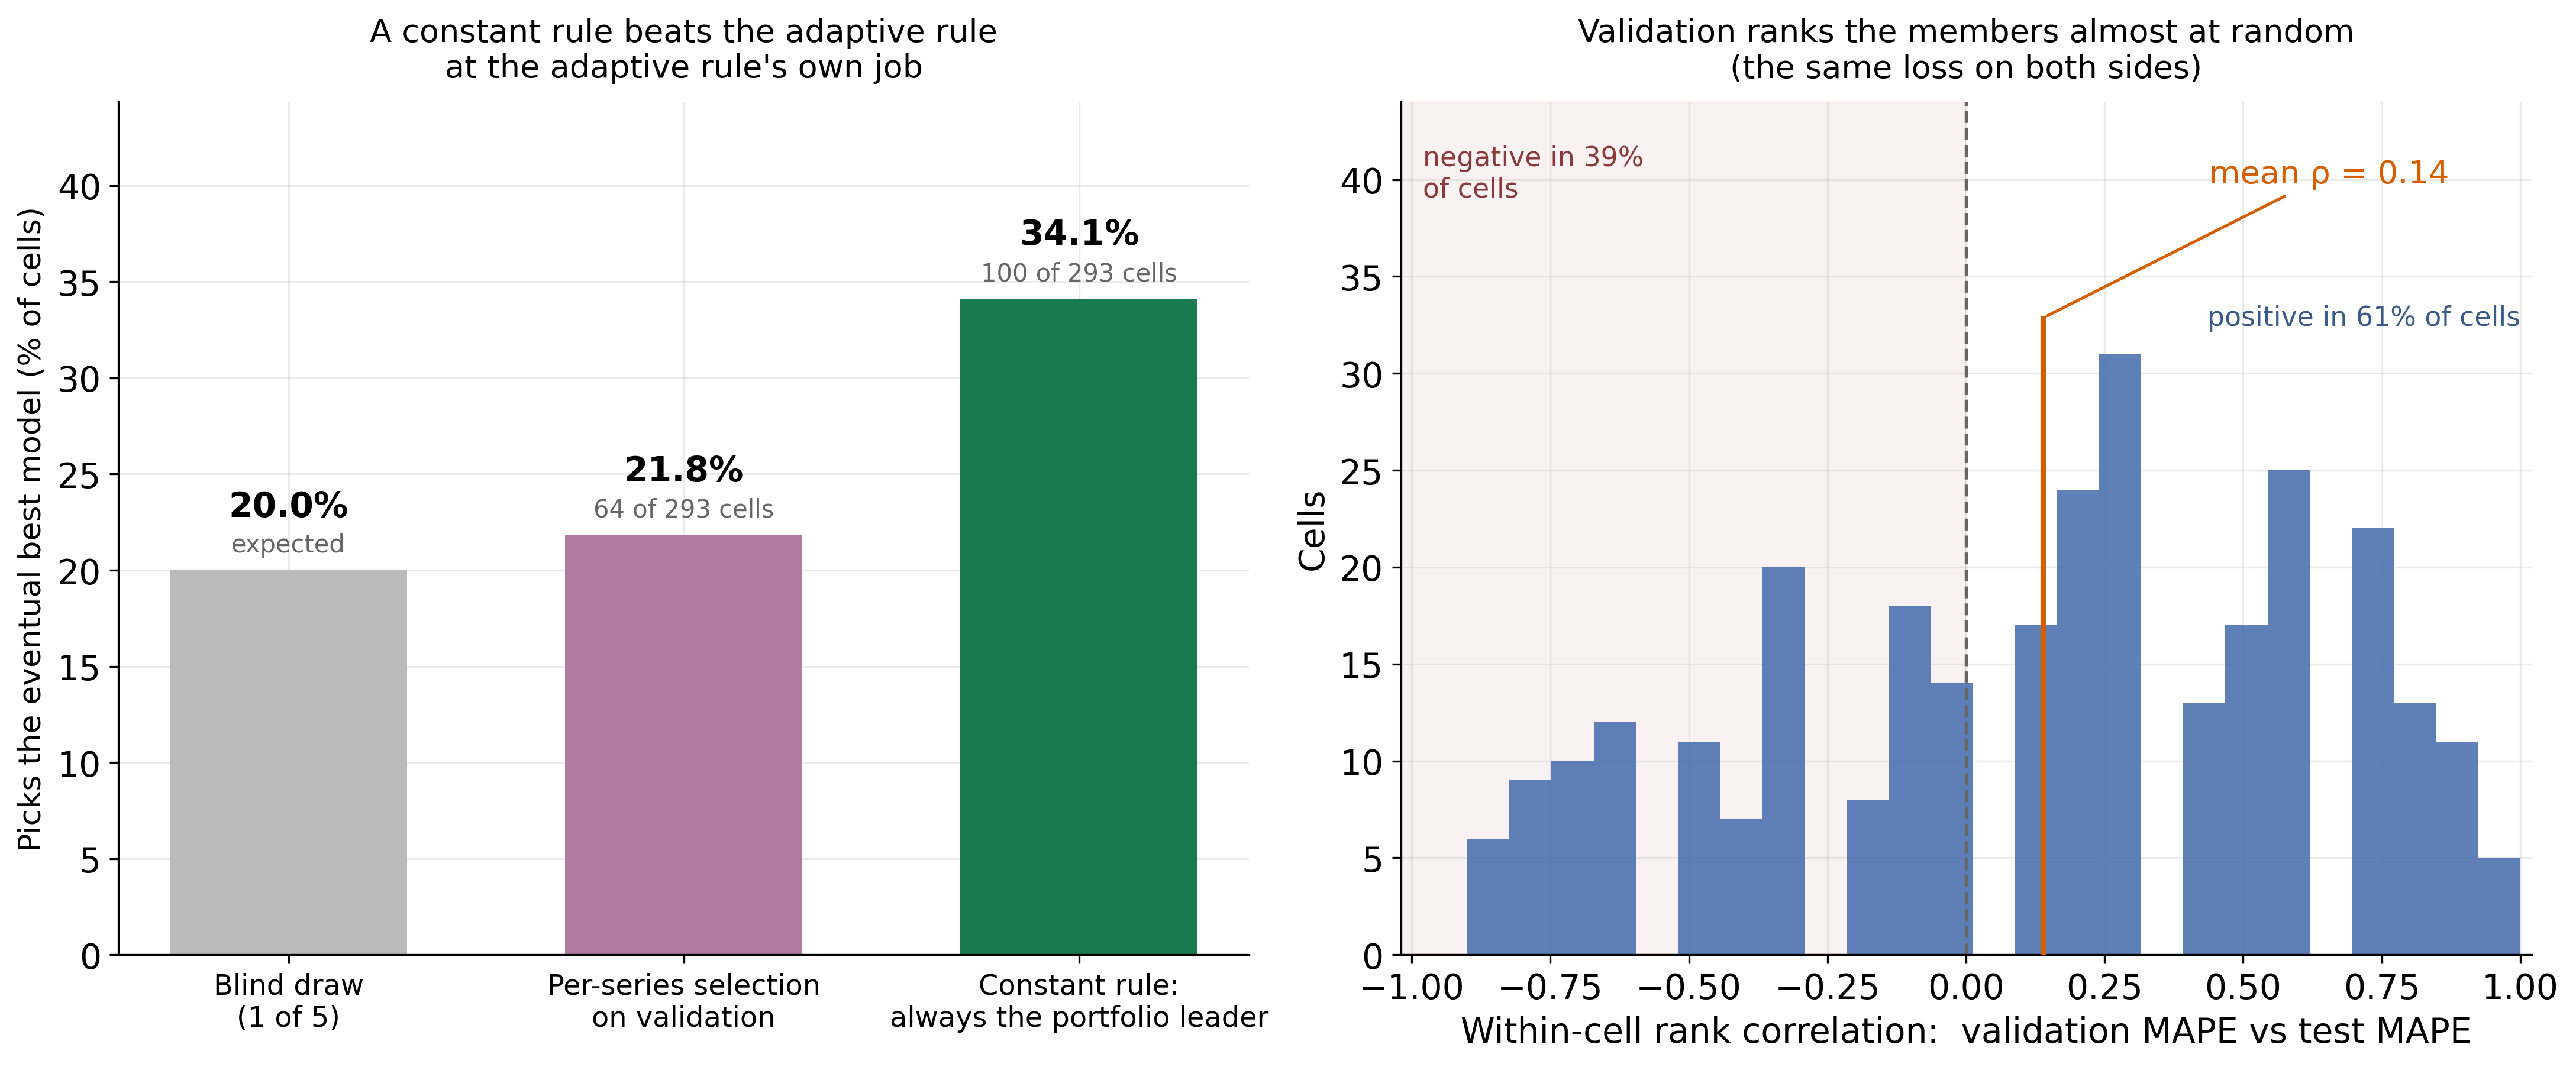
\includegraphics[width=0.98\textwidth]{../figures/figure02.png}
\caption{Why granularity matters. Left: how often each rule identifies the eventual best model, under the criterion actually used by the selector; the constant rule of always using the portfolio leader beats the adaptive rule that re-decides per series. On a matched loss the adaptive rule's figure rises from 21.8\% to 26.0\%, which does not change the ordering. Right: within-cell rank correlation between validation and test error across the five members, same loss on both sides --- weakly positive on average and negative in 39\% of cells.}
\label{fig:granularity}
\end{figure}

The comparison against a constant rule deserves one qualification, since ``a trivial fixed rule beats the adaptive rule'' is easy to over-read. The 34\% figure belongs to the \emph{best} of the five constant rules, not a typical one. Averaged over the five, a constant rule attains mean RelMAE 0.901 and a 20.0\% hit rate (Table~\ref{tab:constant}), so per-series selection at 0.803 and 21.8\% beats four of the five and beats the average comfortably. Selection does add value over ignorance. What it does not do is add as much value as knowing which single model to fix on --- and the point of this paper is that such knowledge is obtainable from the same validation data, provided enough is pooled.

\begin{table}[htbp]\centering\small
\caption{Constant rules against per-series selection, 293 cells. Hit rate is the share of cells in which the rule's model is the best of the five on the test window. The average row is the unweighted mean over the five constant rules, which is what a practitioner with no information would expect. Per-series selection beats four of the five and the average, and loses only to the best.}
\label{tab:constant}
\begin{tabular}{lcc}
\toprule
Constant rule (always use this model) & Mean RelMAE & Hit rate \\
\midrule
CatBoost & 0.747 & 34.1\% \\
BayesianPyMC & 0.835 & 20.1\% \\
NeuralProphet & 0.940 & 16.0\% \\
Prophet & 0.960 & 18.4\% \\
SARIMAX & 1.025 & 11.3\% \\
\midrule
Average over the five constant rules & 0.901 & 20.0\% \\
Per-series validation-selected & 0.803 & 21.8\% \\
Ensemble (Trimmed) & 0.737 & --- \\
\bottomrule
\end{tabular}
\end{table}

Compared directly, full-panel selection beats per-series selection in 104 of the 160 cells where the two differ, by a mean of 0.056 across all 293 cells ($p \approx 5.8\mathrm{e}{-4}$, and stronger at the series and organisation levels): the granularity effect measured without the ensemble as intermediary. The Nemenyi procedure does not separate them (rank gap 0.84 against CD 1.52), which is expected, since it corrects for all 55 pairwise comparisons and is computed on the 99 series rather than the 293 cells.

Read this way, the finding is a statement about estimation variance rather than about combining versus choosing. All the strategies face the same question --- which model should produce this forecast --- and differ only in how much data they bring to it. Per-series selection estimates a five-way ranking from a single short validation window. Portfolio selection estimates the same ranking from many validation windows at once. Combination declines to estimate the ranking at all. Only the first is dominated, which is what one expects if the binding constraint is the precision of the estimate rather than the act of choosing. Figure~\ref{fig:vsselection} shows the per-cell distribution of the ensemble's advantage over per-series selection, and Section~\ref{sec:pooling} traces what happens between the two extremes of pooling.

\begin{figure}[htbp]\centering
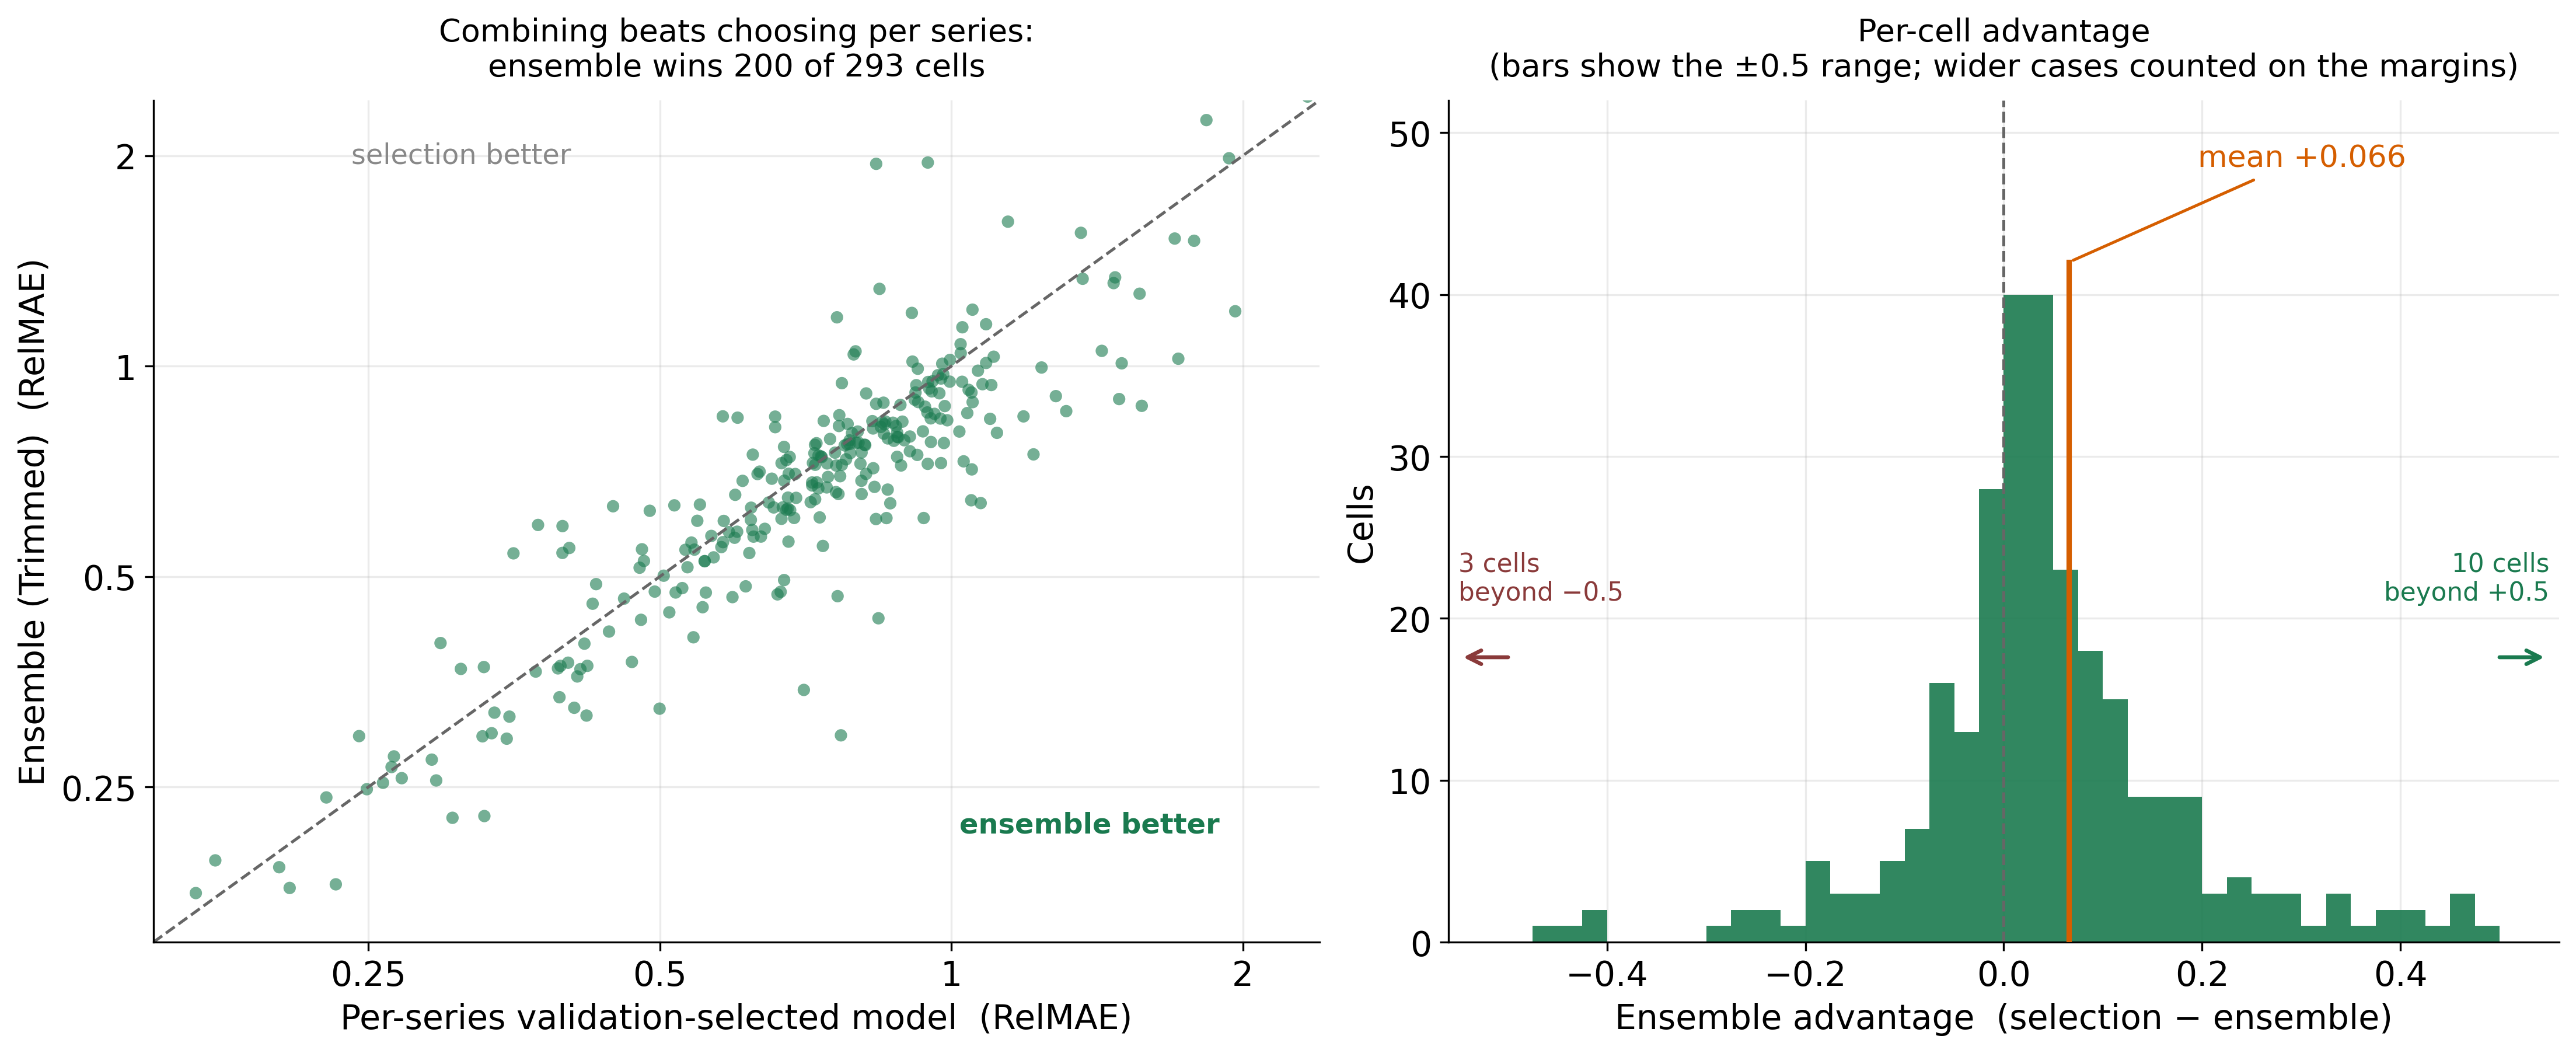
\includegraphics[width=0.98\textwidth]{../figures/figure03.png}
\caption{Trimmed ensemble versus the per-series validation-selected model. Left: per-cell RelMAE on log axes; points below the diagonal favour the ensemble, which wins 200 of 293 cells. Right: distribution of the per-cell advantage over the $\pm 0.5$ range, with the 13 wider cases counted on the margins rather than clipped into the end bins.}
\label{fig:vsselection}
\end{figure}

\subsection{Statistical significance}
\label{sec:significance}

Cells within a series are not independent, since the three rolling origins share training history and series-level noise, so a rank test run across all 293 cells would treat as independent observations that are not. We therefore average each method's per-cell ranks within a series first and run the comparison on the 99 series. This is the same unit the headline comparisons use (Section~\ref{sec:units}), and it is the conservative choice: it widens the critical difference from 0.88 to 1.52 and so makes every claim of separation harder to sustain.

On that basis a Friedman test over the eleven ranked methods rejects equal performance ($\chi^2 = 376.9$, $p \approx 8\mathrm{e}{-75}$). The Nemenyi critical difference at $\alpha = 0.05$ is $\mathrm{CD} = 1.52$ rank positions. The four combination rules hold the best average ranks (4.36--4.62), ahead of CatBoost, which is also full-panel selection (5.29), then per-series selection (6.13), the four remaining single models (6.23--7.76) and Theta (8.87). Three conclusions follow (Figure~\ref{fig:cd}).

First, the trimmed mean we recommend separates from per-series selection, with a rank gap of 1.64 against a critical difference of 1.52. The equal-weighted mean and the inverse-error-weighted combination separate as well, at 1.61 and 1.77. This is the significance result attached to the practical claim.

Second, the combination rules are statistically superior to Theta and to the four single models other than CatBoost, whose ranks trail the top group by more than CD in every case.

Third, the comparison against CatBoost, and so against full-panel selection, is not resolved in the ensembles' favour. Every combination rule falls inside the critical difference against it, the largest gap being 0.93 for the Weighted ensemble against a CD of 1.52. The Weighted ensemble also pays for its rank advantage with a worse tail: the difference in maxima between Trimmed and Weighted is $-1.10$ with a series-bootstrap 95\% interval of $[-2.24, -0.63]$, which excludes zero, as does the corresponding difference in maximum regret. For our reference method we therefore claim parity rather than superiority against a well-chosen single model --- noting that parity is obtained here without having to identify that model, which is the practical asymmetry between the two.

\begin{figure}[htbp]\centering
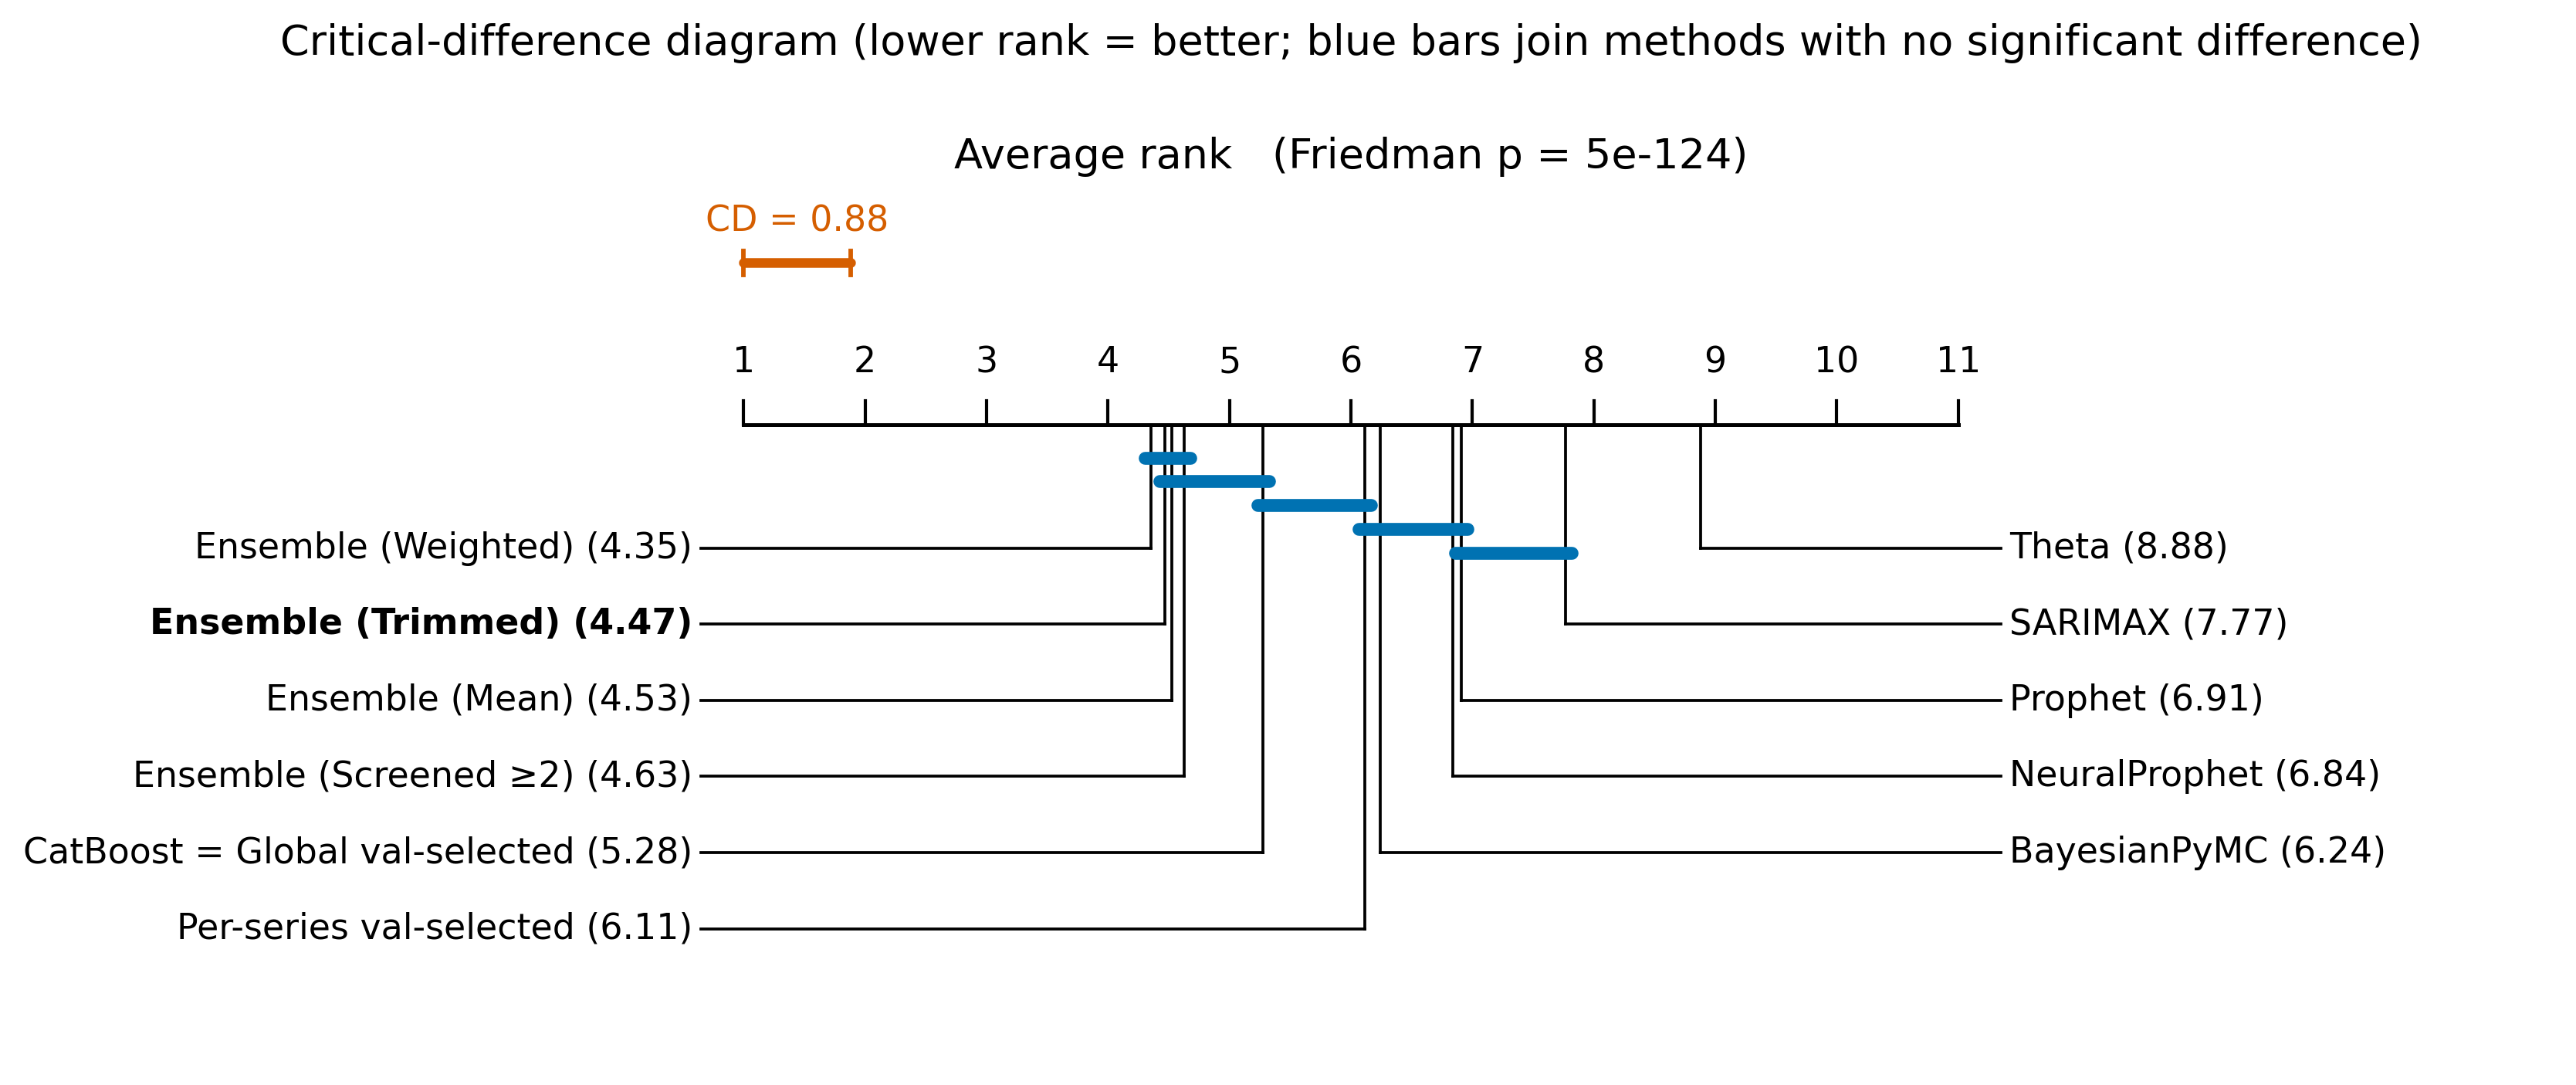
\includegraphics[width=0.90\textwidth]{../figures/figure04.png}
\caption{Nemenyi critical-difference diagram over the eleven ranked methods, computed on ranks averaged within series and tested across the 99 series rather than the 293 cells. Lower rank is better; a bar joins methods that are statistically indistinguishable. Full-panel portfolio selection is not drawn separately, since on this corpus it resolves to the CatBoost forecast path.}
\label{fig:cd}
\end{figure}

The pairwise tests tell the same story with effect sizes attached. Against per-series selection the Holm-adjusted $p$ is $5.7\mathrm{e}{-9}$ with rank-biserial 0.41; against Theta, SARIMAX, Prophet, NeuralProphet and the Bayesian model the adjusted $p$-values range from $4\mathrm{e}{-33}$ to $1\mathrm{e}{-12}$, with rank-biserial 0.50 to 0.82; against CatBoost the adjusted $p$ is 0.059 with rank-biserial 0.16 and a mean difference of $-0.010$; and against the other three combination rules all adjusted $p$-values are 1.00. In the CatBoost comparison we draw attention to the effect size rather than the $p$-value: one per cent of benchmark error would not justify a change of method even had it reached significance.

\subsection{Consistency and tail behaviour}
\label{sec:tails}

The ensembles' most-claimed advantage is dependability, and we hold that claim to the same standard as the mean claims. Single models are boom-or-bust: SARIMAX and Prophet occasionally produce extreme errors even after the non-negativity constraint, and Theta more often still. Against those methods the tail advantage is large and unambiguous. Against per-series selection every point estimate favours the ensemble and one quantile is resolvable. Against a well-chosen single model it is not established at all.

The levels in Table~\ref{tab:tails} put the trimmed ensemble below CatBoost at P90 (1.04 against 1.07) and at the maximum (2.63 against 2.72), but those gaps do not survive interval estimation and we do not rest anything on them (Figure~\ref{fig:tailboot}). Reporting the difference of the point estimates with a basic bootstrap interval, P90 is $-0.027$ $[-0.168, +0.022]$; P95 is $+0.001$ $[-0.335, +0.274]$; P99 is $+0.231$ $[-0.141, +0.582]$, CatBoost being lower there; and the maximum is $-0.085$ $[-0.839, +0.386]$. Every interval contains zero and the point estimates change sign across quantiles. A maximum over 293 cells is a single observation and should not carry a headline claim in a paper otherwise careful about inference.

Against per-series selection the same procedure gives $-0.070$ $[-0.178, +0.141]$ at P90, $-0.246$ $[-0.480, +0.069]$ at P95, $-0.556$ $[-1.371, -0.153]$ at P99, and $-0.378$ $[-0.863, +0.094]$ at the maximum. Every point estimate favours the ensemble and the P99 interval excludes zero. One methodological sensitivity is worth stating. Computing the interval as the percentile range of bootstrapped differences instead, which is the more common convention, makes P95 the resolvable quantile and P99 not. Which single quantile clears the threshold is therefore method-dependent, and the defensible summary is that the ensemble's tail advantage over per-series selection is consistent in direction at every quantile and marginally resolvable at one of them. We report the point-estimate difference with a basic interval as the primary convention because it is the only one whose reported difference is guaranteed to agree in sign with the levels in Table~\ref{tab:tails}.

\begin{figure}[htbp]\centering
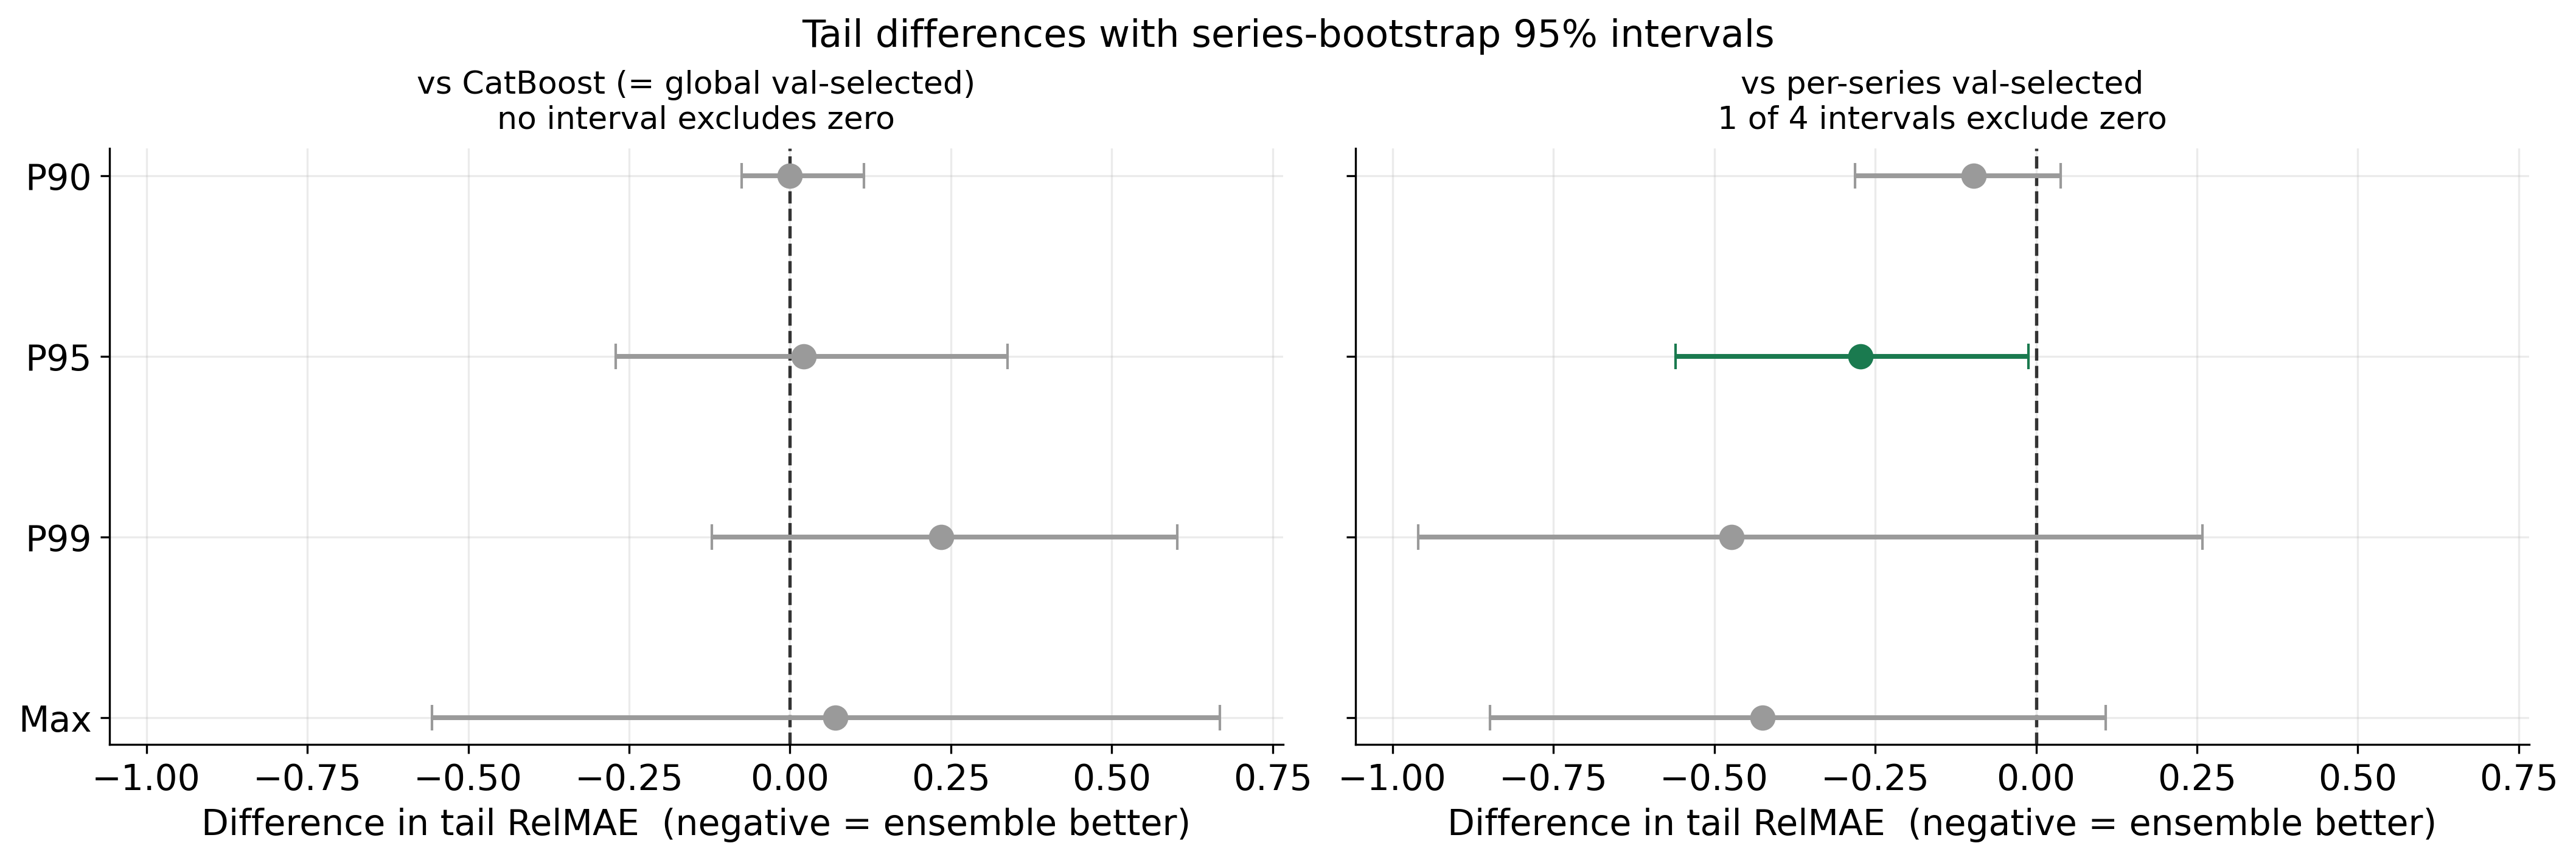
\includegraphics[width=0.98\textwidth]{../figures/figure05.png}
\caption{Tail differences between the trimmed ensemble and each competitor, with series-bootstrap 95\% intervals; green marks an interval excluding zero. Against CatBoost no interval excludes zero and the sign of the point estimate is not stable across quantiles. Against per-series selection every point estimate favours the ensemble.}
\label{fig:tailboot}
\end{figure}

Two results are not in doubt on any reading, and they are the ones we would act on. The first is regret. The trimmed ensemble has the lowest mean regret to the per-cell oracle of all twelve methods (0.10, against 0.11 for CatBoost and 0.17 for per-series selection) and the lowest maximum regret (1.59, against 2.14 and 2.17), and it beats every single model outright --- negative regret --- in 65 of 293 cells (22.2\%), so it is not merely hedging towards the middle of its members. We hold this to the same standard as everything else: against per-series selection the mean-regret difference is $-0.066$ with a series-clustered interval of $[-0.096, -0.033]$ and is resolvable, while against CatBoost it is $-0.010$ $[-0.038, +0.017]$ and is not. The defensible claim is therefore that the ensemble carries the lowest regret of any method tested and demonstrably lower regret than per-series selection, not that it carries lower regret than a well-chosen single model.

The second is rank frequency, and it is the sharpest practical contrast in the study (Figure~\ref{fig:rankdist}). CatBoost is the single best method in 13.0\% of cells against the trimmed ensemble's 8.9\%, so on a plurality of individual cells the single model is preferable. But CatBoost lands in the worst three of the eleven ranked methods in 17.4\% of cells against the ensemble's 1.0\%. At equal typical accuracy, the two methods differ by a factor of seventeen in how often they deliver a bad quarter. We are precise about what that is and is not: it is a statement about the frequency of poor \emph{ranks} among the eleven methods compared here, not about the magnitude of the tail, which Section~\ref{sec:tails} shows this design cannot resolve against CatBoost. A frequency of bad outcomes and a size of bad outcomes are different quantities, and only the first is established. The distinction is not a technicality: the two statistics answer different questions. How often a method produces a poor outcome relative to its alternatives is what a planning process accumulates over many cycles; how large the single worst outcome is matters to a practitioner exposed to one catastrophic event. On this corpus the ensemble's advantage is in the first and not demonstrably in the second.

The mechanism behind the frequency result is the error diversity of Section~\ref{sec:diversity}. A single model's extreme error is transmitted to every series in the panel with nothing to damp it. For the trimmed mean the output is the average of the middle two members, so an extreme output requires at least two of the four to be extreme in the same direction at the same time --- not merely one, as for a single model, though not all four either, since the two outermost members are discarded before the average is taken. At a mean pairwise signed-error correlation of 0.63 the members disagree enough that this is uncommon, and the 1.0\% worst-three frequency is the empirical measure of how uncommon. Whether the same asymmetry appears on another panel depends on its error correlation structure, which is why Section~\ref{sec:scope} lists that correlation as one of the three diagnostics to run before adopting the recommendation.

\begin{figure}[htbp]\centering
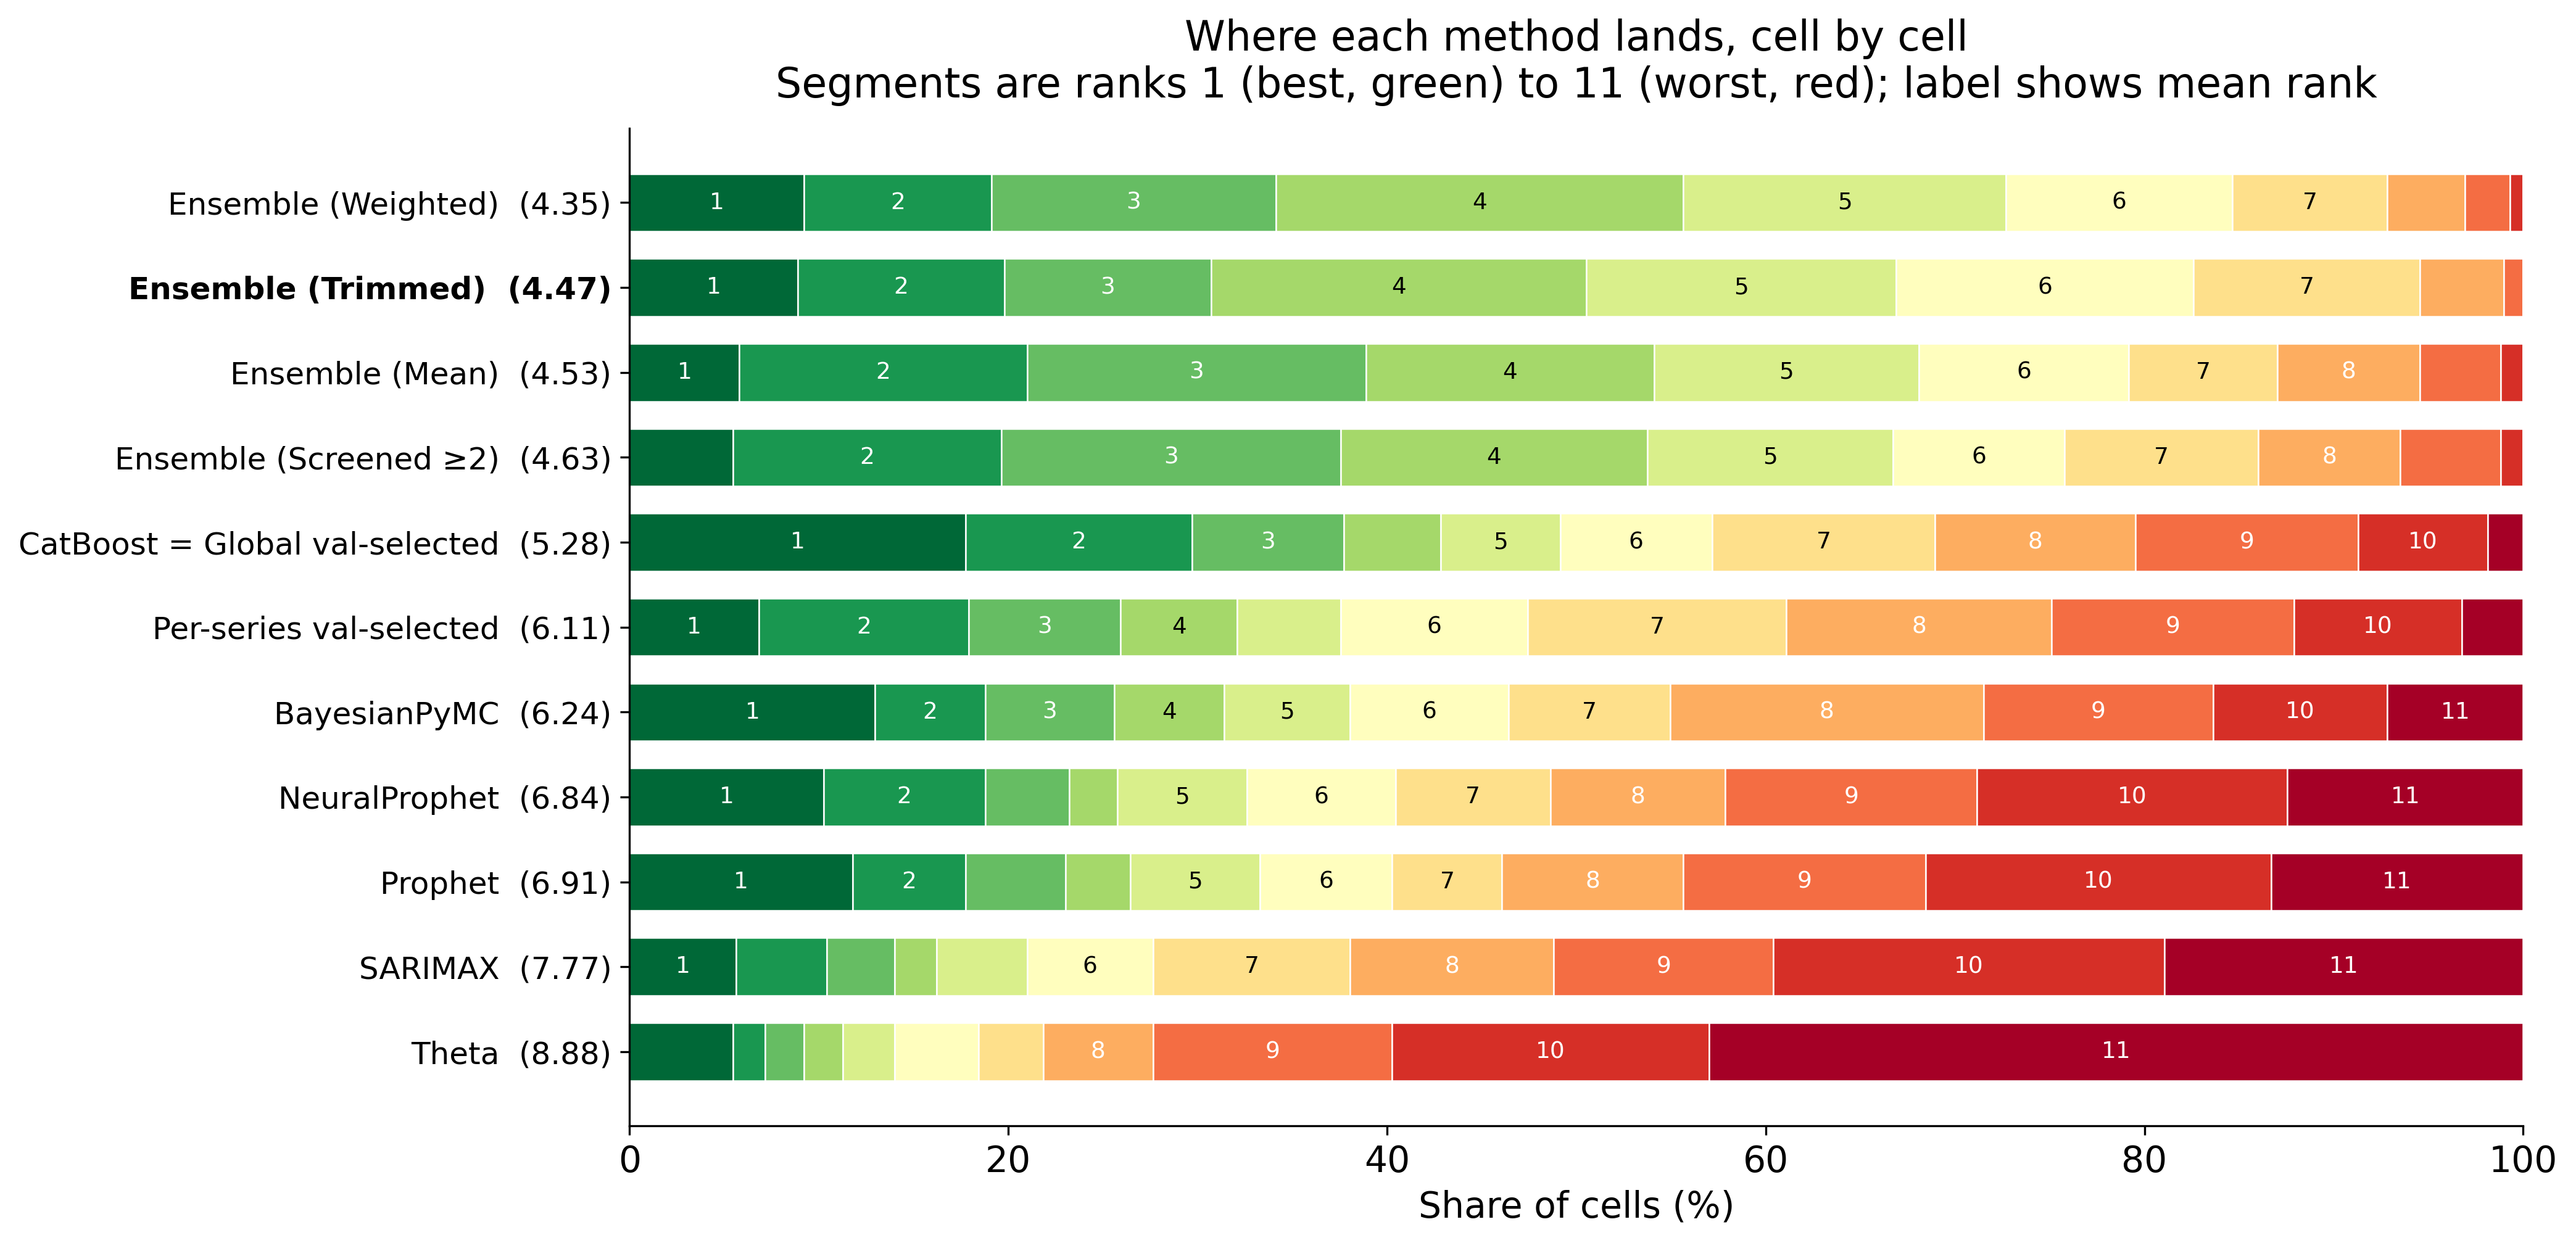
\includegraphics[width=0.92\textwidth]{../figures/figure06.png}
\caption{Per-method rank distribution over the 293 cells (rank 1 = best). Ties contribute half their weight to each adjacent rank; per-series selection is tied with its chosen base model in every cell by construction, which is why it records no outright rank-1 share, and the Mean and Screened combinations coincide in 218 cells. Mean ranks are shown beside each label and match Table~\ref{tab:central}.}
\label{fig:rankdist}
\end{figure}

\begin{figure}[htbp]\centering
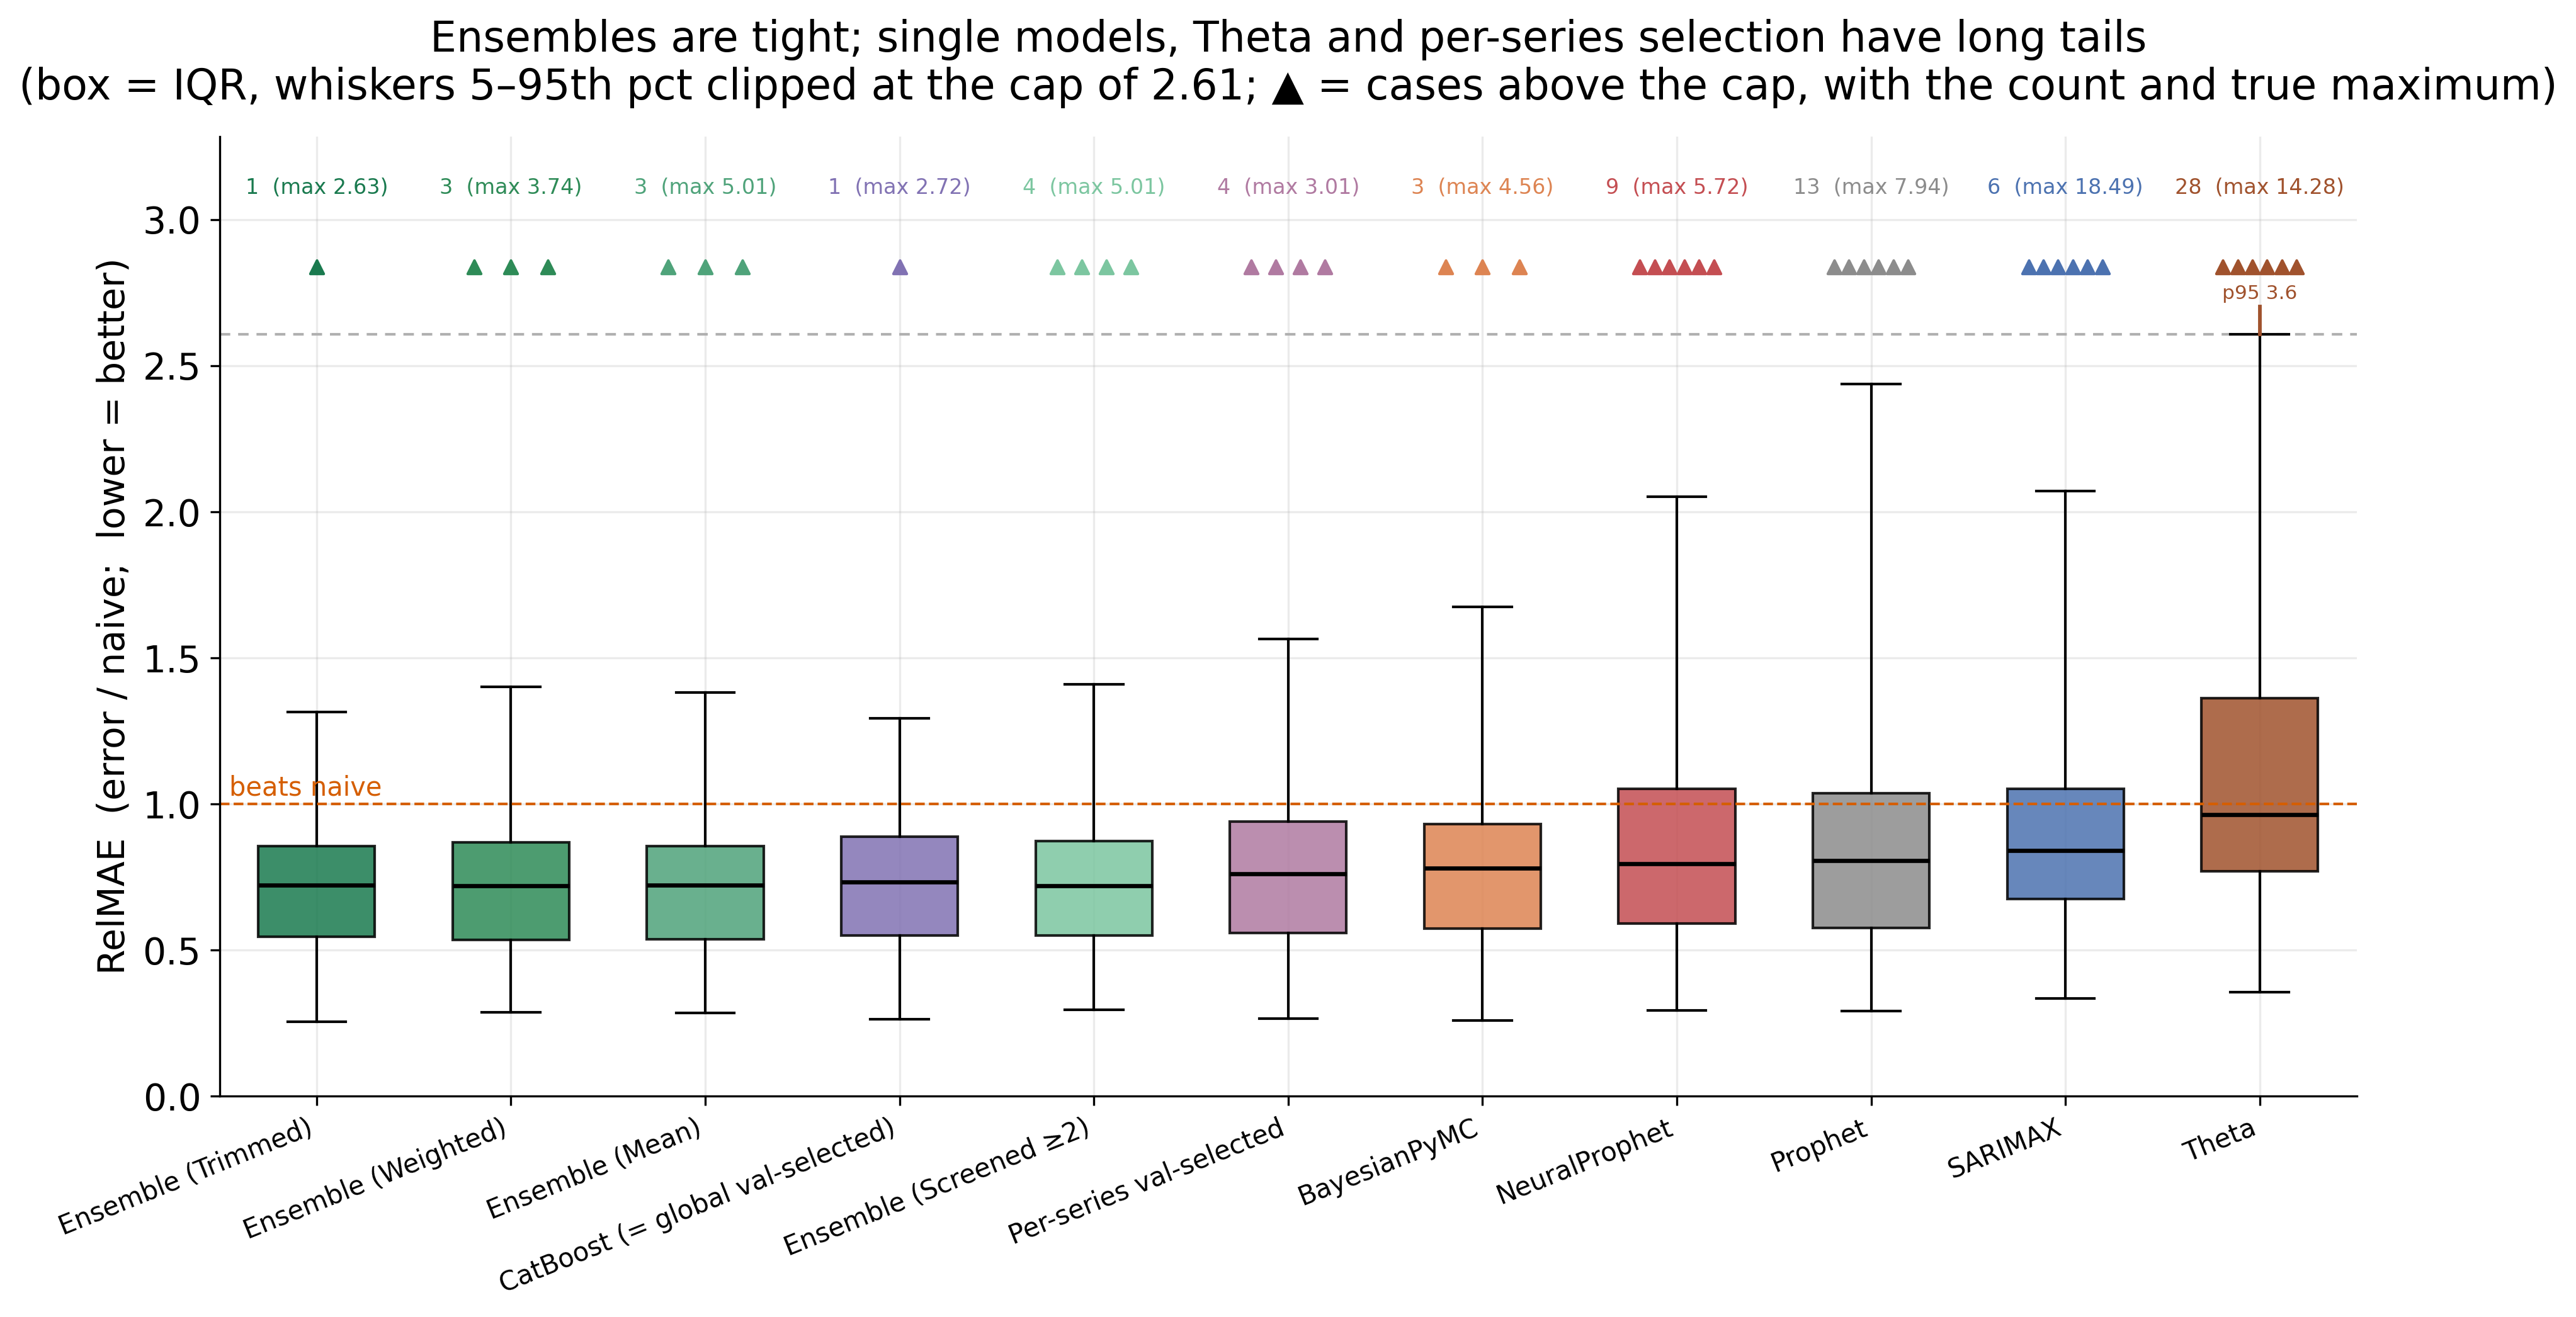
\includegraphics[width=0.92\textwidth]{../figures/figure07.png}
\caption{Per-cell RelMAE distribution by method, ordered by geometric mean as in Table~\ref{tab:central}. Box = interquartile range, whiskers = 5th--95th percentile, clipped at an axis cap of 2.61; triangles mark cells above the cap, labelled with the count and the true maximum.}
\label{fig:dist}
\end{figure}

\begin{figure}[htbp]\centering
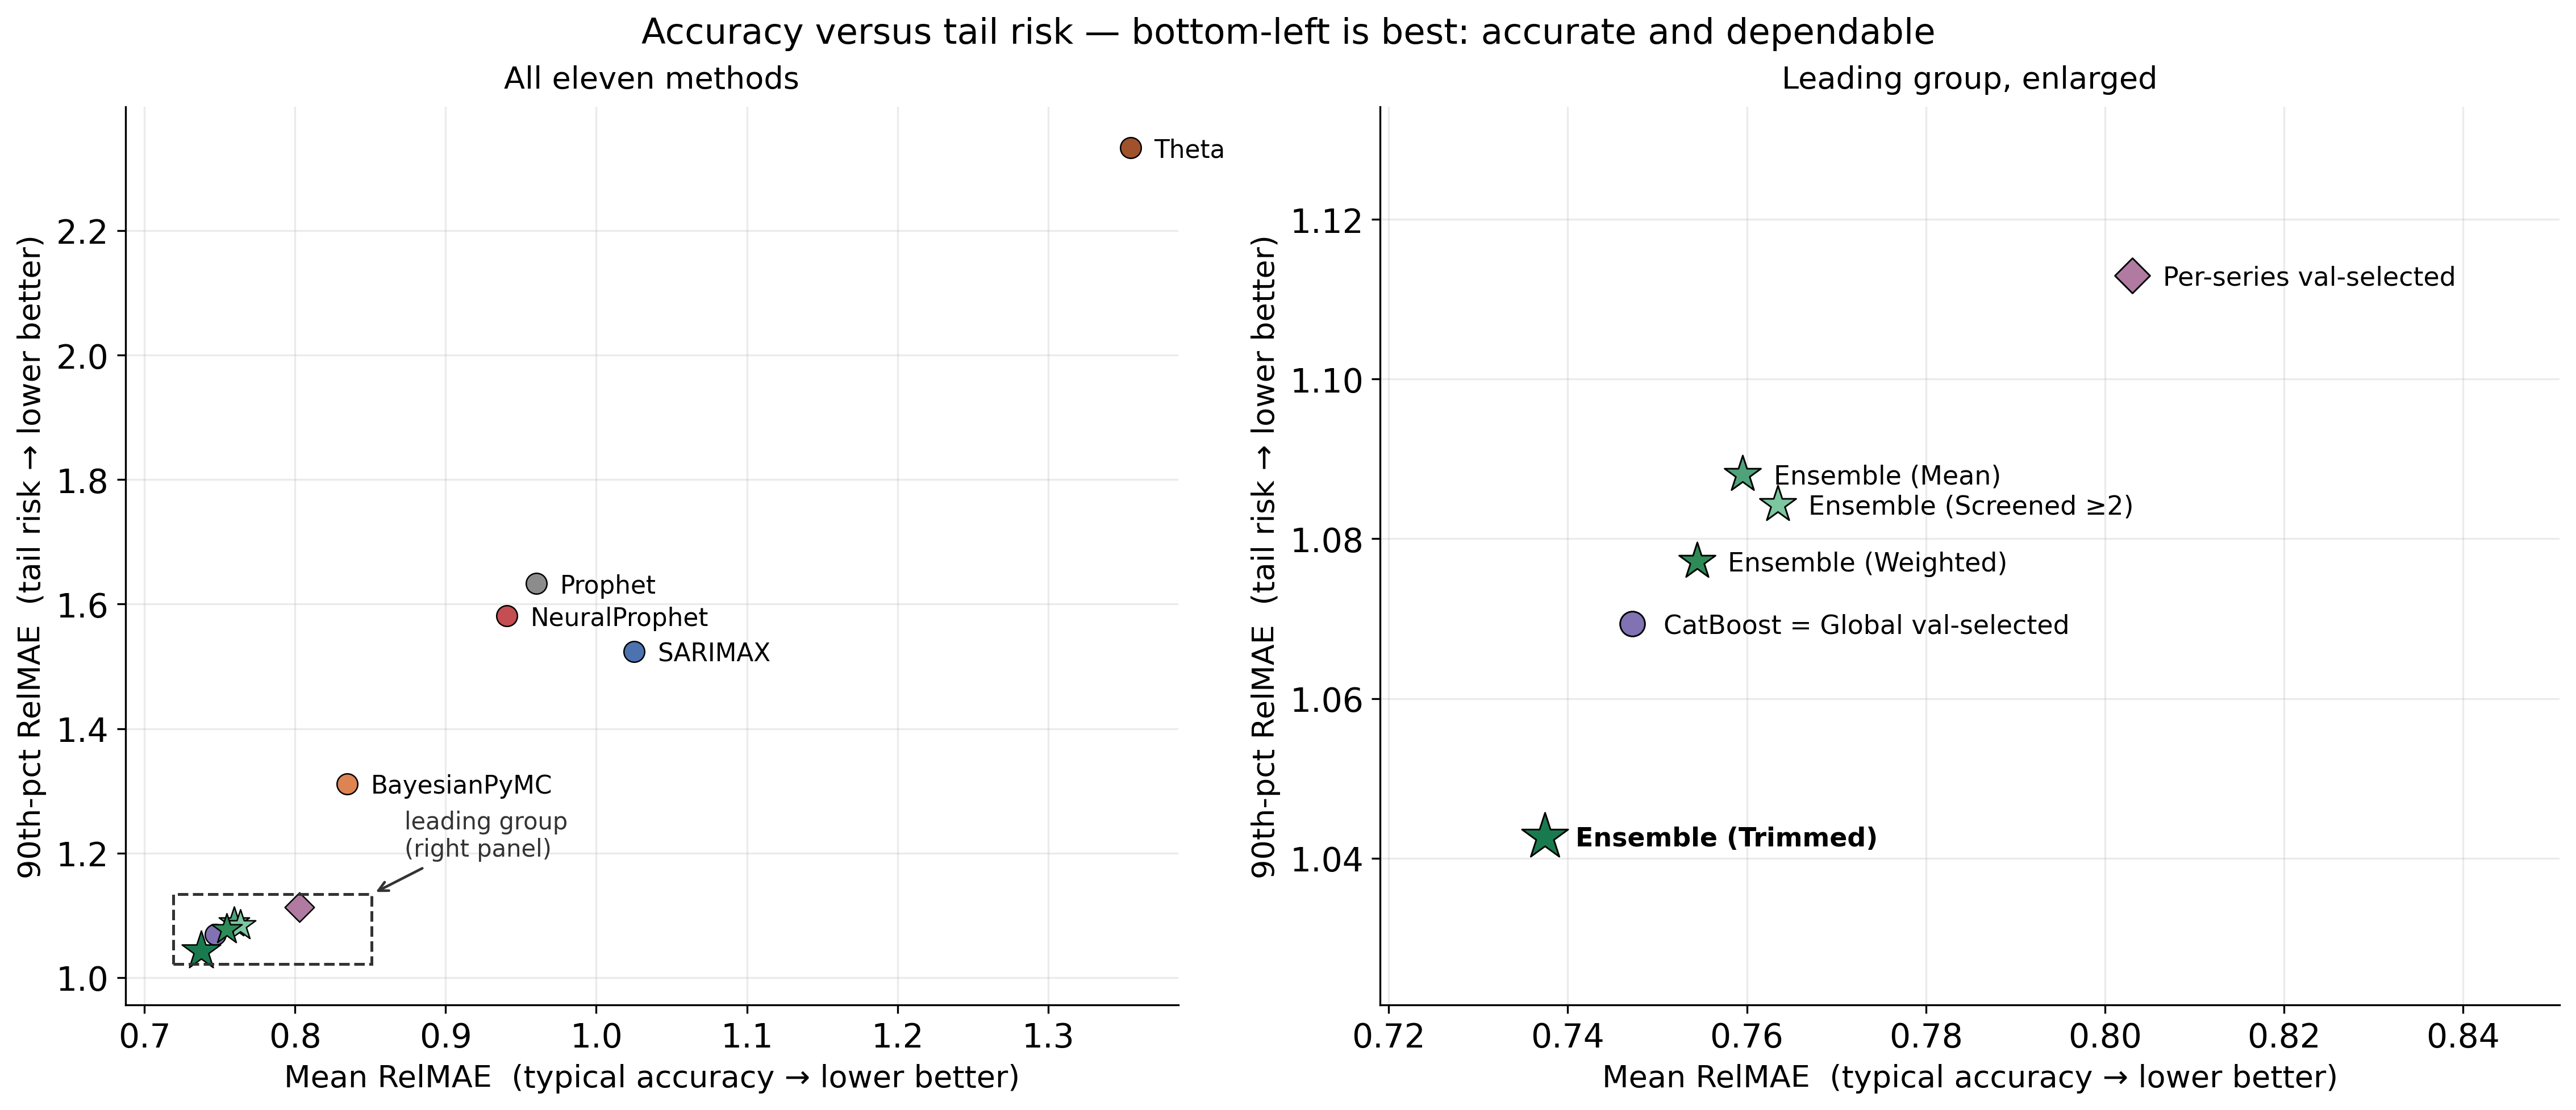
\includegraphics[width=0.98\textwidth]{../figures/figure08.png}
\caption{Mean RelMAE versus 90th-percentile RelMAE. Bottom-left is best: accurate and dependable. Left, all eleven methods; the dashed box marks the leading group. Right, that group enlarged. Stars are combination rules, the diamond is per-series selection, circles are single models. The tail axis is P90; at P99 the ordering of the ensemble and CatBoost reverses, as Table~\ref{tab:tails} records.}
\label{fig:tradeoff}
\end{figure}

\subsection{Horizon, or training length?}

Because test windows vary from 73 to 210 days, the panel appears to support a question the aggregate tables cannot answer: does the ranking of methods depend on how far ahead they forecast? Splitting the cells into terciles of test-window length gives an apparently clear answer (Table~\ref{tab:horizon}) --- the ensemble is ahead of CatBoost at short horizons, level in the middle, and behind at long ones --- inviting the interpretation of a horizon interaction.

\begin{table}[htbp]\centering\small
\caption{Mean RelMAE by tercile of test-window length. The ensemble's advantage over per-series selection holds in every tercile (0.088, 0.037, 0.071). Its position relative to CatBoost varies across terciles, but test-window length and training length grow together --- the fourth column --- so the variation cannot be attributed to horizon.}
\label{tab:horizon}
\begin{tabular}{lcccccccc}
\toprule
Tercile & Cells & Mean test & Mean train & Trimmed & CatBoost & Per-series & Theta & Oracle \\
\midrule
Short & 98 & 89 d & 477 d & 0.761 & 0.800 & 0.849 & 1.601 & 0.665 \\
Mid & 97 & 124 d & 664 d & 0.753 & 0.754 & 0.790 & 1.427 & 0.637 \\
Long & 98 & 175 d & 940 d & 0.699 & 0.688 & 0.770 & 1.037 & 0.600 \\
\midrule
Total & 293 & 129 d & 695 d & 0.737 & 0.747 & 0.803 & 1.355 & 0.634 \\
\bottomrule
\end{tabular}
\end{table}

We keep this table in the main text rather than an appendix for a specific reason: the pattern in it is one a reader would reconstruct from the aggregate figures and then misread. Reporting it next to the control that dissolves it is more useful than omitting it and leaving the confound undocumented.

That interpretation does not survive the obvious control. Validation and test windows are each 12\% of series length, so test-window length and training-set length are almost the same variable: their logs correlate at 0.887, giving a variance inflation factor of 4.7, and the long-horizon tercile has nearly twice the training history of the short one. Regressing the per-cell RelMAE difference (trimmed minus CatBoost) on both jointly, with standard errors clustered on series, assigns essentially nothing to horizon and what little signal there is to history: the coefficient on log test length is $-0.0019$ (clustered $t = -0.02$) and on log training length $+0.0665$ (clustered $t = +0.77$), with a joint Wald statistic of 1.45. Neither term is significant, but the horizon coefficient is indistinguishable from zero once history is controlled for.

The honest statement is that this design cannot separate the two, and that the pattern in Table~\ref{tab:horizon} is at least as consistent with a training-length effect --- a gradient-boosted learner with covariates becoming reliably strong once it has enough history --- as with anything about lead time. We therefore report the confound rather than a horizon interaction. What the table does establish, and what matters for the argument, is that the advantage over per-series selection is present in all three terciles.

\subsection{Why combination helps: error diversity}
\label{sec:diversity}

Combination pays off only when members disagree. Pooling all 37,884 test observations and scaling each cell's errors by its seasonal-naive MAE, the mean pairwise Pearson correlation of signed forecast error across the five base models is 0.63, ranging from 0.46 (SARIMAX--NeuralProphet) to 0.81 (CatBoost--Bayesian) (Figure~\ref{fig:corr}). Members are positively but far from perfectly correlated, though 0.63 places this panel closer to the low-diversity boundary of Section~\ref{sec:scope} than the headline results suggest. The structure is interpretable: SARIMAX is the most distinct member (0.46--0.55 against all others), while CatBoost, the Bayesian model, and the additive-decomposition family form a more tightly coupled block (0.65--0.81). We report signed-error correlation deliberately: it is the quantity the Bates--Granger diversification argument concerns. Correlating per-cell error magnitudes instead gives a lower number (0.47) but answers a different question, whether some cells are uniformly hard.

A correlation of 0.63 is high enough that the residual disagreement should be quantified. For the equal-weighted combination of the four de-duplicated members the squared error decomposes exactly as $\mathrm{MSE}_{\text{comb}} = \mathrm{mean}_j\, \mathrm{MSE}_j - D$, where $D$ is the mean squared dispersion of the members about their own average. Averaged over the 293 cells and scaled by the squared naive MAE, the average member's MSE is 2.30 and $D$ is 0.72: combination removes 31\% of the average member's squared error, leaving 1.57. The decomposition is exact for the equal-weighted mean only; the trimmed mean is not an affine combination and its benefit is not captured by it.

Trimming adds a second and distinct mechanism. Its value has usually been described as protection against whichever member is aberrant on a given day, and the data support a more precise statement. Across the four de-duplicated members, the shares of trimmed slots are SARIMAX 28.6\%, the Bayesian model 22.9\%, CatBoost 22.5\%, and the additive representative 26.0\%, against 25\% each under uniformity. Since two of four members are trimmed each period, SARIMAX sits at an extreme in roughly 57\% of periods and each other member in roughly 45--52\%: every member takes its turn at the edge, and trimming is not a disguised way of dropping one weak member.

Within a cell, however, the aberrant member is highly persistent. The identity of the trimmed-high member changes from one day to the next in only 15.6\% of consecutive period pairs, so it is unchanged on 84.4\% of days, and the median cell contains an unbroken run of 40 days on which the same member occupies the high slot. This is the opposite of day-to-day rotation. What trimming buys in this corpus is therefore closer to an automatic, per-cell exclusion of whichever member is systematically misbehaving on that series and period, applied without anyone having to identify it, than to a high-frequency defence against transient outliers; the rotation that matters happens across cells rather than across days. That reading is consistent with the ablation of Section~\ref{sec:ablation}, which finds the benefit concentrated in the tail, and it remains the regime in which robust averages are predicted to help \citep{jose2008,kourentzes2019}.

\begin{figure}[htbp]\centering
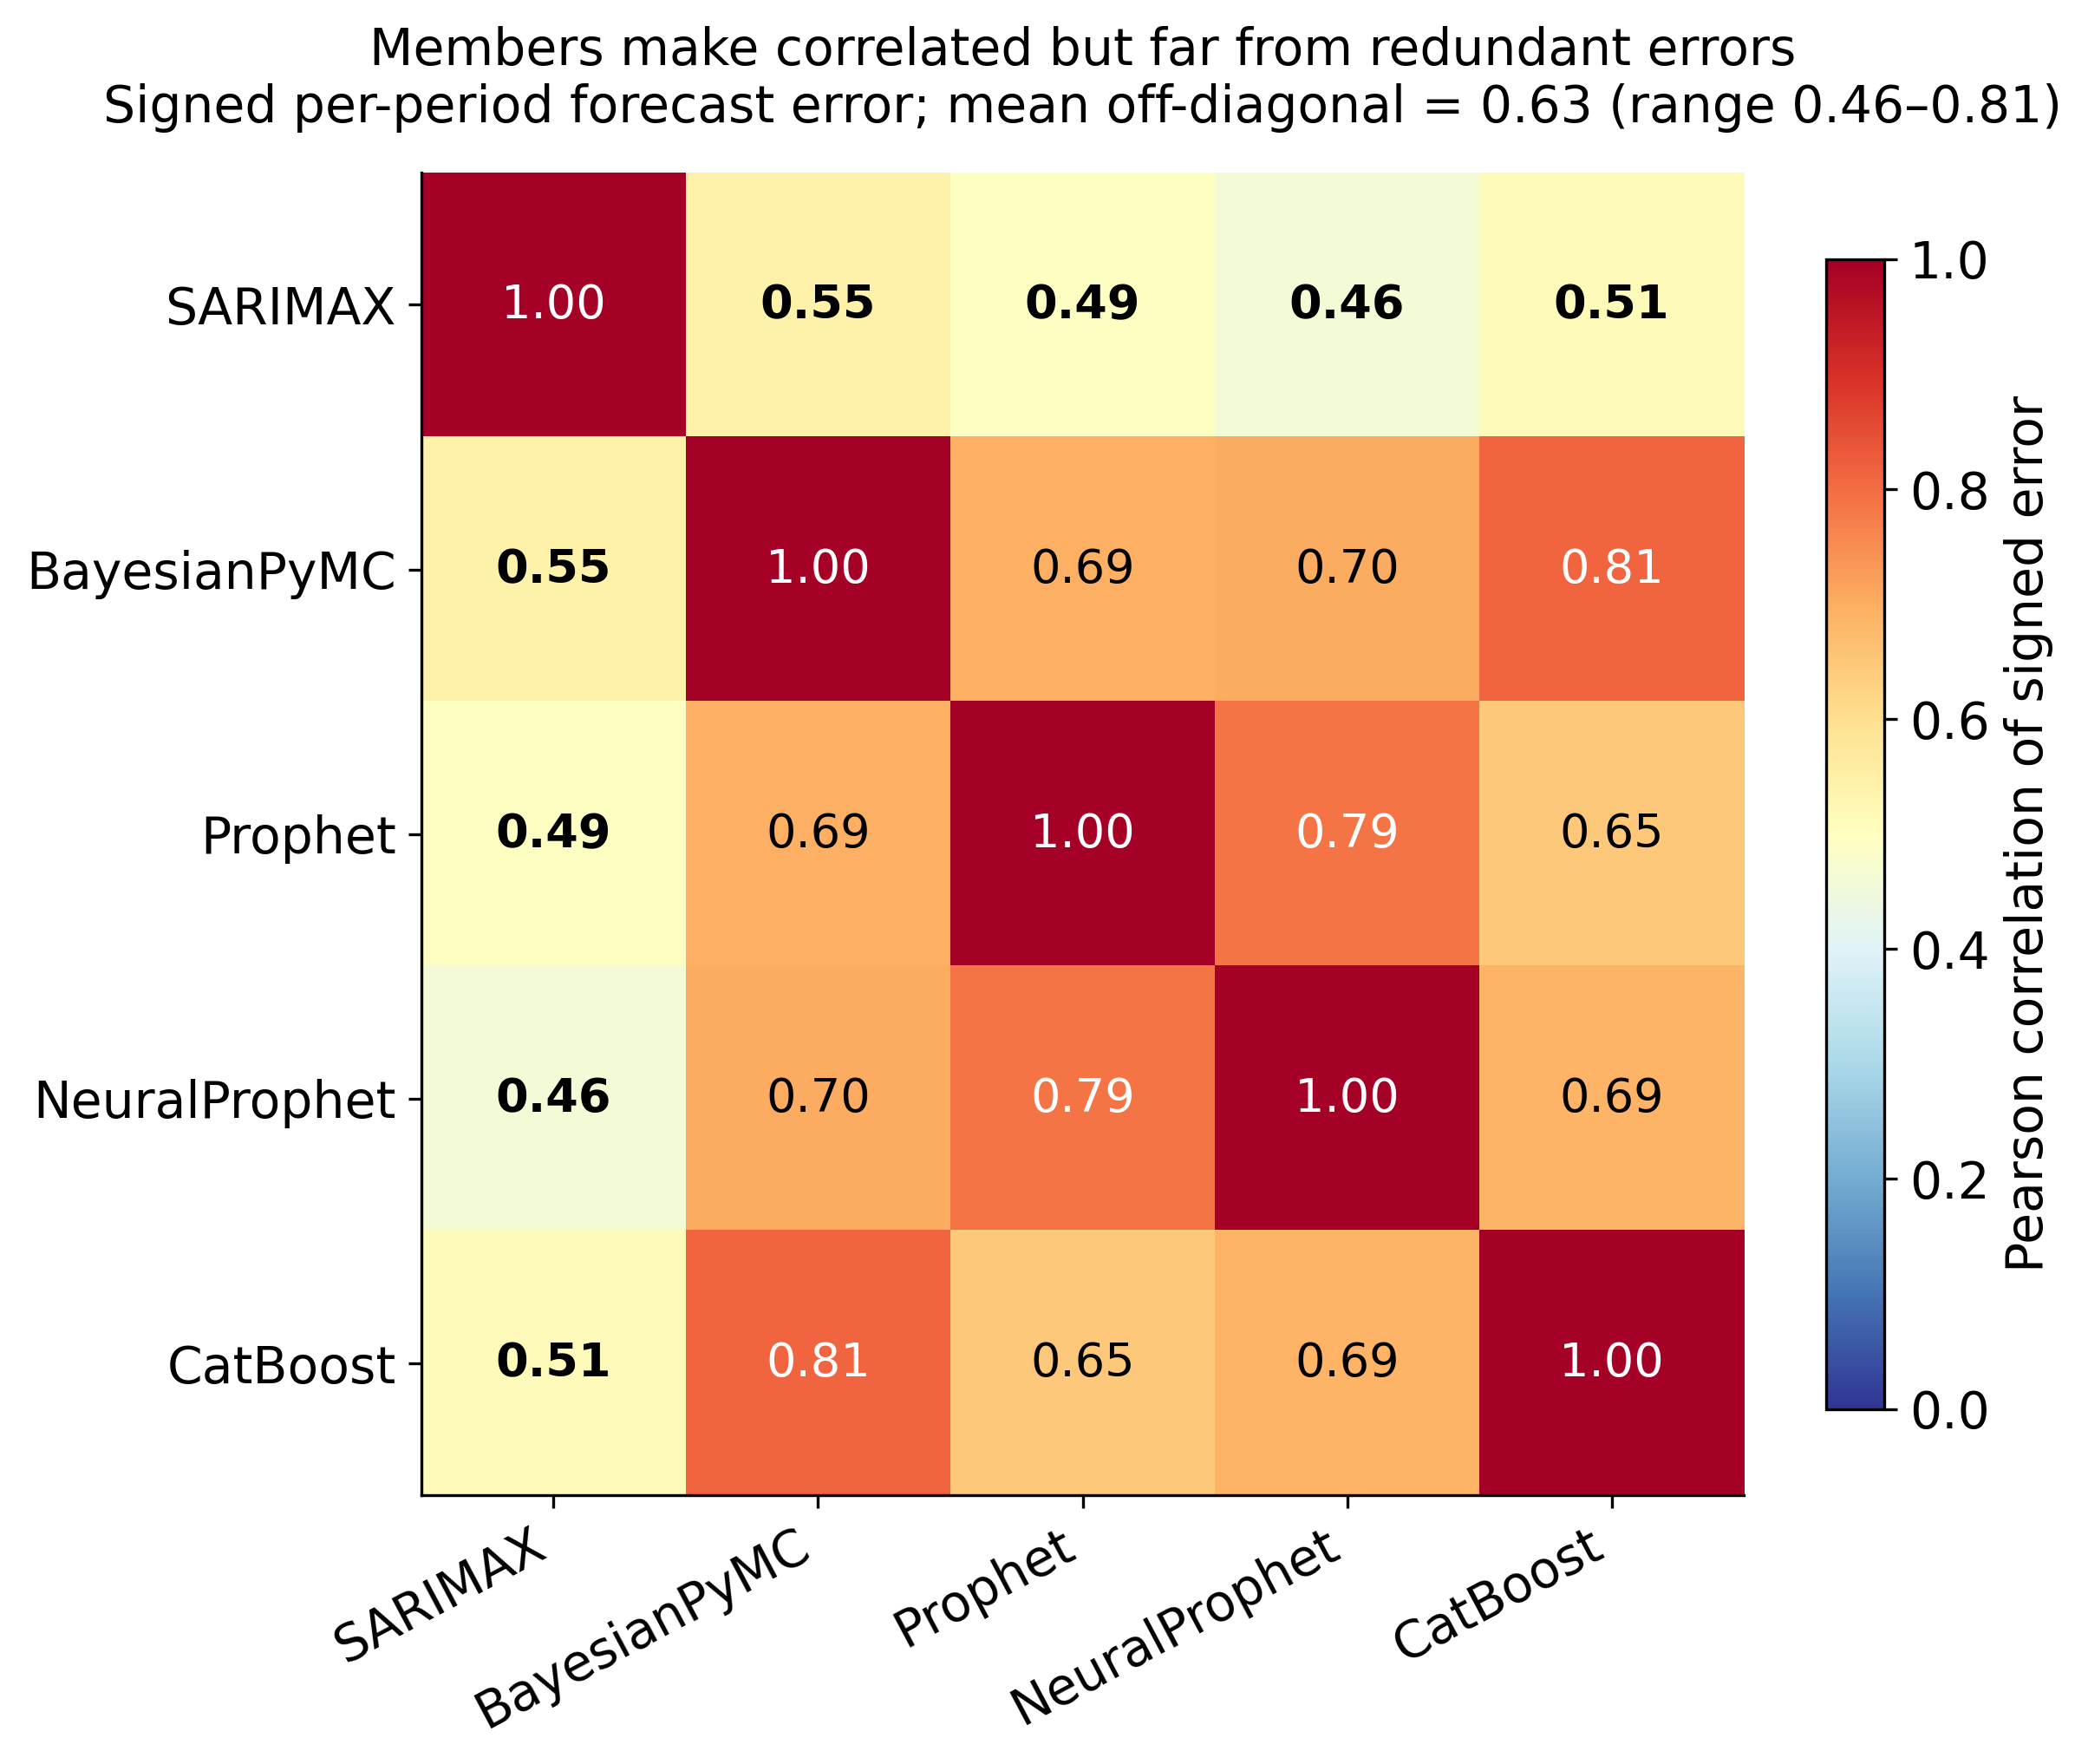
\includegraphics[width=0.62\textwidth]{../figures/figure09.png}
\caption{Pearson correlation of signed per-period forecast error across base models, pooled over all test observations and scaled within cell. Low off-diagonal values indicate complementary errors.}
\label{fig:corr}
\end{figure}

\subsection{Does family de-duplication earn its place?}
\label{sec:ablation}

Section~\ref{sec:dedup} justifies collapsing Prophet and NeuralProphet to one representative on structural grounds. A structural rationale is not evidence, so we test the construction by re-running the trimmed mean and the equal mean over all five members and comparing against the four de-duplicated members (Table~\ref{tab:dedup}), holding everything else fixed.

\begin{table}[htbp]\centering\small
\caption{Family de-duplication ablation on the same 293 cells. The final column reports the difference in maxima between the de-duplicated and five-member versions of each rule, with a series-bootstrap 95\% interval, so that the tail claim is held to the standard Section~\ref{sec:tails} applies elsewhere.}
\label{tab:dedup}
\begin{tabular}{lcccccc}
\toprule
Combination & Members & Mean & Median & P90 & Max & Max diff.\ vs 5-member \\
\midrule
Trimmed, de-duplicated (ref.) & 4 & 0.737 & 0.723 & 1.04 & 2.63 & $-0.64$ $[-1.45, -0.17]$ \\
Trimmed, all members & 5 & 0.747 & 0.718 & 1.06 & 3.28 & \\
Mean, de-duplicated & 4 & 0.760 & 0.723 & 1.09 & 5.01 & $+1.35$ $[+1.35, +3.80]$ \\
Mean, all members & 5 & 0.764 & 0.713 & 1.12 & 3.66 & \\
\bottomrule
\end{tabular}
\end{table}

Before reading the table, one feature of it needs naming, because the two rows differ in more than membership. At four members the trimmed mean is the median; at five it is the mean of the middle three. The comparison therefore varies the operator alongside the member set, and the two have to be separated before either can be attributed. Holding the operator fixed at the median and varying only membership gives 0.737 for the four de-duplicated members against 0.750 for all five, so membership is worth 0.013. Holding membership fixed at five and varying only the operator gives 0.750 for the median against 0.764 for the equal mean, so the robust centre is worth another 0.013. Both contribute, in similar measure, and the 0.737 against 0.747 comparison in the table is the sum of the two rather than a membership effect alone.

With that separation in hand, the result is mixed. On typical accuracy de-duplication does little: the de-duplicated trimmed mean is better in 143 of 293 cells, a Wilcoxon $p$ of 0.72, and its median is marginally worse (0.723 versus 0.718); the same holds for the equal mean (139 of 293, $p = 0.66$). Any claim that de-duplication substantially improves typical accuracy is not supported by this corpus.

What it delivers is a better tail for the trimmed combination: the maximum falls from 3.28 to 2.63, a difference of $-0.64$ $[-1.45, -0.17]$ excluding zero, with P99 moving $-0.20$ $[-0.63, +0.02]$ in the same direction. This is coherent with the mechanism, since removing one of two correlated members makes it harder for that methodology to occupy both extreme slots and so survive trimming. The effect does not carry over to the equal mean, whose maximum is worse when de-duplicated, 5.01 against 3.66, a difference of $+1.35$ $[+1.35, +3.80]$ that also excludes zero. That the two rules move in opposite directions, both resolvably, locates the benefit in the trimming step rather than in membership as such. The interval is pre-specified; the mechanism offered for the asymmetry is a reading of an observed pattern and should be treated as post-hoc.

We therefore retain family de-duplication on three grounds, in order of strength: it improves the tail of the recommended method, resolvably; it is structurally principled; and it is cheaper, since one member fewer must be scored at forecast time. We do not claim it improves typical accuracy, and a reader who rejects the structural argument and is indifferent to the tail loses very little by combining all five members.

That variant is worth stating on its own account, because it settles a question the reference construction leaves slightly open. The trimmed mean over the de-duplicated set is described throughout as estimating nothing, and in its combination step it does not; but the de-duplication itself resolves the additive family on validation MAPE, so one validation-driven decision per cell survives. The trimmed mean over all five members removes even that. It uses no validation quantity at any point --- no ranking, no weights, no threshold, no family resolution --- and attains mean RelMAE 0.747 with median 0.718, level with the full-panel selection strategy at 0.747 and behind the reference ensemble by 0.010. A rule with no estimated component anywhere in it therefore matches a single model chosen with the benefit of the entire portfolio's validation evidence. That is the paper's central point in its simplest form, and it costs one member's worth of extra scoring at forecast time.

\subsection{Robustness to the unit of aggregation}
\label{sec:units}

Cells within a series share training history and series-level noise, and series within an organisation may share reporting conventions and demand shocks. Our view is that a territory series is the right independent unit, but this is a judgement, so we make the conclusions independent of it (Table~\ref{tab:units}).

\begin{table}[htbp]\centering\small
\caption{Every headline comparison at three units of aggregation. Wilcoxon signed-rank; counts are cells (series, organisations) in which the trimmed ensemble is better. The comparison against per-series selection survives at all three units; the comparison against full-panel selection does not survive past the cell level. The final row compares per-series and full-panel selection directly; its cell count is out of the 160 cells in which they differ, the two coinciding in the remaining 133.}
\label{tab:units}
\begin{tabular}{lccc}
\toprule
Comparison & Cells ($N = 293$) & Series ($n = 99$) & Organisations ($n = 65$) \\
\midrule
Trimmed vs Per-series selection & 200/293, $p \approx 1.1\mathrm{e}{-9}$ & 77/99, $p \approx 1.0\mathrm{e}{-7}$ & 50/65, $p \approx 1.6\mathrm{e}{-5}$ \\
Trimmed vs Full-panel selection & 165/293, $p \approx 0.015$ & 58/99, $p \approx 0.074$ & 35/65, $p \approx 0.53$ \\
\midrule
Mean RelMAE, Trimmed & 0.737 & 0.736 & 0.746 \\
Mean RelMAE, Per-series sel. & 0.803 & 0.803 & 0.821 \\
Mean RelMAE, Full-panel sel. & 0.747 & 0.749 & 0.749 \\
Mean difference vs per-series & $-0.066$ & $-0.067$ & $-0.075$ \\
\midrule
Full-panel vs Per-series sel. & 104/160, $p \approx 5.8\mathrm{e}{-4}$ & 62/99, $p \approx 2.4\mathrm{e}{-4}$ & 46/65, $p \approx 9.3\mathrm{e}{-5}$ \\
\bottomrule
\end{tabular}
\end{table}

The central claim holds at every unit, with the effect size essentially unchanged and the $p$-value never rising above $2\mathrm{e}{-5}$. The comparison against full-panel selection degrades monotonically and is entirely absent at the organisation level, which is why Sections~\ref{sec:granularity} and \ref{sec:significance} report it as a tie. The direct comparison between the two selection strategies strengthens as the unit coarsens, which is the granularity effect showing through most clearly at the most conservative unit. Confidence intervals widen only slightly under organisation resampling, consistent with within-organisation dependence being real but modest.

\subsection{Robustness across industries}
\label{sec:verticals}

A per-vertical comparison invites counting the verticals in which the ensemble leads, but with bootstrap intervals attached that count is not interpretable. Of the eight named verticals with at least three series, two have fewer than six and cannot support an interval at all --- with three series the bootstrap has only ten distinct resamples, which is why Arts \& Entertainment shows the tightest interval despite being the smallest group (Figure~\ref{fig:verticals}). Among the six that can, the difference excludes zero in two, Business \& Industrial and Home \& Garden, both favouring the ensemble.

We state the direction of the other four rather than only that they include zero. In Apparel, the largest vertical at 21 series, the point estimate favours CatBoost by 0.055 with an interval of $[-0.002, +0.125]$ that only just includes zero, and in Beauty \& Fitness it favours CatBoost by 0.055 with a much wider interval; in Food \& Drink and Sports it favours the ensemble by 0.028 and 0.023. So the ensemble does not lead everywhere, and in the largest single vertical it trails. Per-vertical sample sizes of 6 to 21 series do not resolve differences of this magnitude in either direction, and we present the figure as an illustration of dispersion rather than evidence of within-vertical superiority.

That dispersion carries an implication worth stating, because it cuts in the direction opposite to the one the Apparel row first suggests. The sign of the ensemble-minus-CatBoost difference is not stable across verticals: CatBoost is ahead in two and behind in six, on point estimates that mostly cannot be resolved. If the identity of the better strategy varies across subpopulations of a single corpus --- collected the same way, screened the same way, forecast the same way --- then committing an entire panel to one model is a bet that the aggregate ranking holds in every corner of it, and this corpus gives no assurance that it does. A rule that does not have to make that bet is not disadvantaged by the variation. Against per-series selection, by contrast, there is no variation to discuss: the ensemble leads in all eight named verticals and in the unclassified group, without exception.

\begin{figure}[htbp]\centering
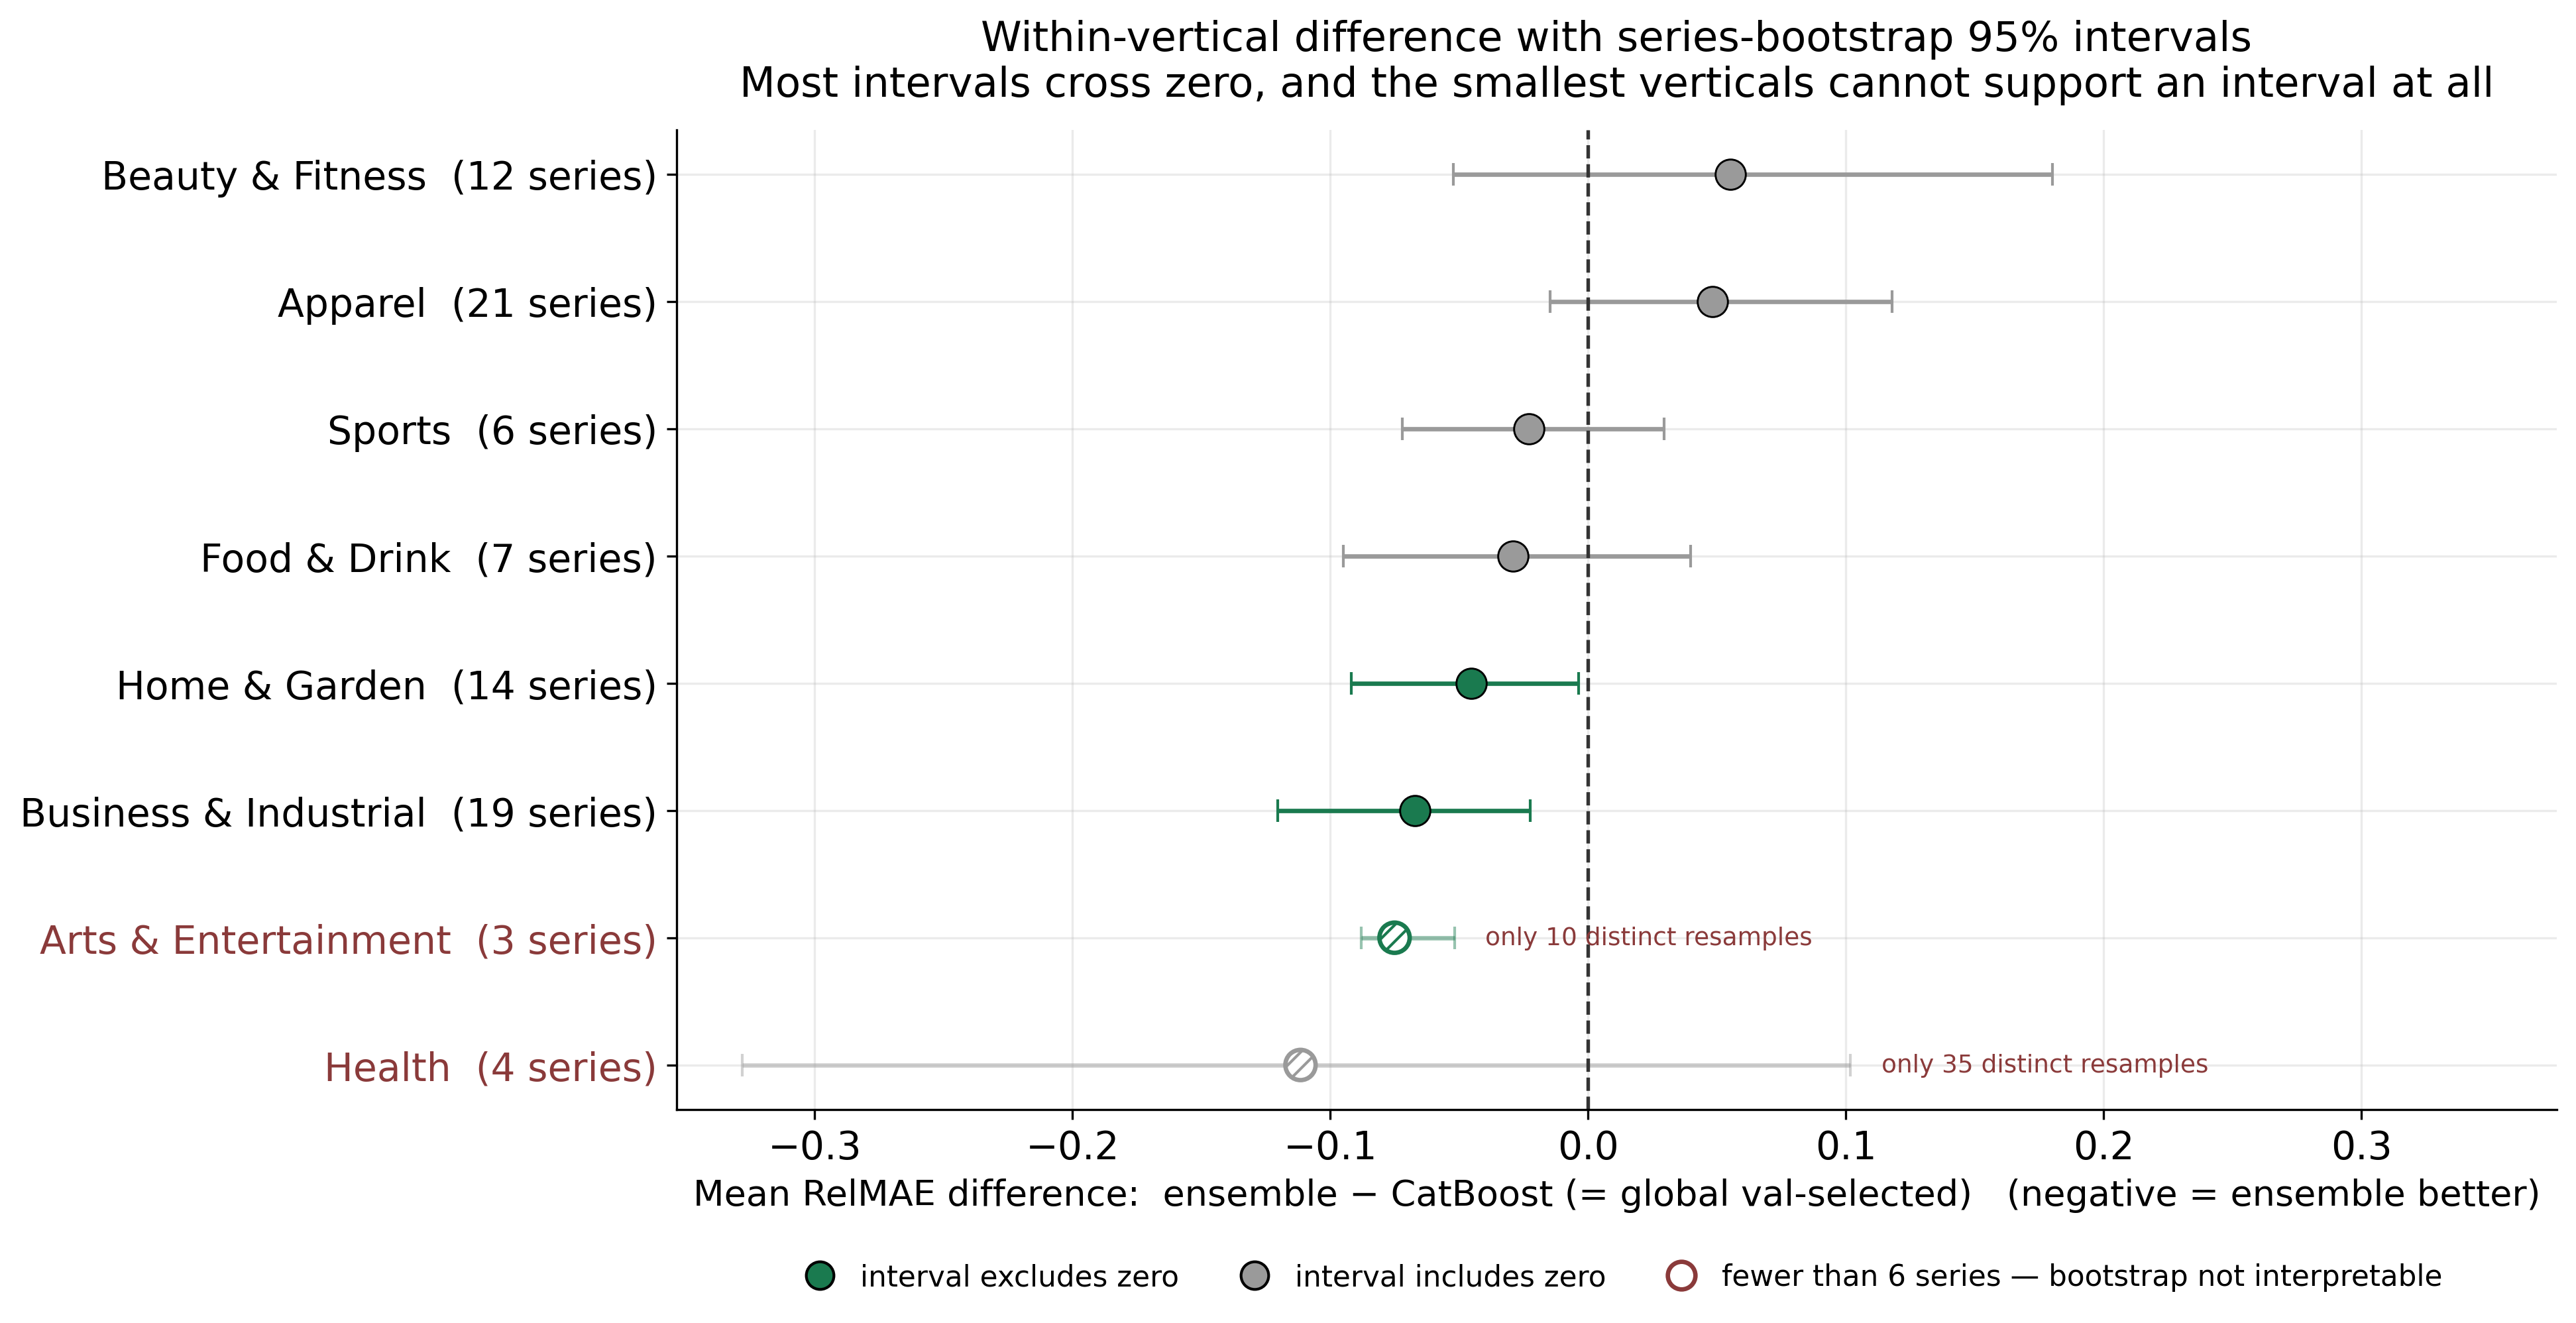
\includegraphics[width=0.98\textwidth]{../figures/figure10.png}
\caption{Within-vertical mean RelMAE difference (ensemble minus CatBoost, which is also full-panel selection) with series-bootstrap 95\% intervals. Named verticals with at least three series are shown; those with fewer than six are drawn hollow, since a bootstrap over so few series has too few distinct resamples to yield a meaningful interval. The 8 unclassified series are omitted from the figure but included in the aggregate comparison reported in the text.}
\label{fig:verticals}
\end{figure}

\subsection{An alternative benchmark}

The seasonal-naive benchmark repeats one fixed week for up to 210 days and so carries no trend, which at these lead times makes it a weak reference. A weak reference flatters every method: it enlarges the denominator, so the RelMAE levels we report are lower than a more demanding benchmark would produce. We therefore recompute the leaderboard against seasonal-naive-with-drift, which adds a linear drift term estimated over all data up to the end of validation. The substitution does not have the intended effect. Drift lowers the benchmark's error in 38\% of cells and raises it in the remaining 62\%, since a trend estimated on history and extrapolated over as much as 210 days is itself high-variance and misfires on series that are flat or that reverse; averaged over the corpus the drift benchmark is therefore the weaker of the two, and mean RelMAE falls slightly for every method --- trimmed 0.737 to 0.725, CatBoost 0.747 to 0.735, per-series selection 0.803 to 0.791, Theta 1.355 to 1.336. What the exercise establishes is not a tougher reference but the ordering's indifference to the choice of one, which is unchanged under either. Within-cell ranks are invariant to the denominator by construction, since the benchmark enters as a common per-cell scale factor, so the Friedman and Nemenyi results are identical under either benchmark and only the cross-cell aggregation weights of the mean columns change. The concern that absolute levels are flattered therefore stands, and the benchmark that would settle it is one carrying annual seasonality, which we note in Section~\ref{sec:caveats} and do not run.

\subsection{How quickly does portfolio selection become reliable?}
\label{sec:pooling}

The full-panel rule of Section~\ref{sec:rules} ranks models using every validation window in the corpus. Within each series that ranking respects time, but across series it does not, since the 99 validation windows sit at different calendar dates. The strategy is therefore best understood as the limit of a rule whose evidence accumulates, and the practically interesting question is how much evidence it needs before it reaches that limit.

We answer it by re-running the rule under an accumulation constraint. At each cell, the selector may rank the five models using only those cells whose validation window had already finished when this cell's forecast was issued. The available evidence grows from a single prior cell at the earliest origins to 292 at the latest, with a median of 147. Everything else is unchanged.

This is a deliberately conservative accounting, and we want to be clear why. The constraint ties the evidence pool to \emph{this study's} origin placement rather than to what a practitioner would actually hold. A cell whose test window begins in 2021 has few completed validation windows largely because most series' origins fall later in calendar time --- an artefact of the research design. A real deployer holding these series in 2021 would have had substantially more history to draw on and could have placed validation windows earlier. The small-pool rows below therefore understate what portfolio selection would achieve in practice, and should be read as a floor rather than an estimate.

Even on that pessimistic accounting, portfolio selection converges quickly (Table~\ref{tab:pooling}). Once roughly 150 cells of evidence have accumulated --- a threshold this corpus reaches for half its cells --- the rule identifies CatBoost in every single cell and attains 0.729 against the ensemble's 0.704 on the same cells, a residual gap of 0.025. Given the full panel, that gap closes to 0.010 and is not resolvable at all, which is the tie of Section~\ref{sec:granularity}. The mid-range behaves as one would expect of an estimator halfway to its limit: at 50--149 prior cells the rule splits between CatBoost and SARIMAX and attains 0.861. Only at the very smallest pools, where fewer than 50 prior cells are available and the constraint is at its most artificial, does the rule select poorly, picking SARIMAX in 44 of 49 cells and attaining 0.981.

\begin{table}[htbp]\centering\small
\caption{Accumulating portfolio selection by the quantity of pooled evidence available at the forecast origin. Cells are grouped by how many other cells had completed their validation window when this cell's forecast was issued. The ensemble column is computed on the same cells in each row, so the gap is a within-group paired comparison. The final row is the full-panel rule of Section~\ref{sec:rules}, the limit the sequence converges to.}
\label{tab:pooling}
\begin{tabular}{lccccc}
\toprule
Evidence at forecast origin & Cells & Model chosen & Portfolio sel. & Trimmed & Gap \\
\midrule
Fewer than 50 prior cells & 49 & SARIMAX 44, CatBoost 5 & 0.981 & 0.847 & $+0.134$ \\
50 to 149 prior cells & 100 & CatBoost 58, SARIMAX 42 & 0.861 & 0.731 & $+0.130$ \\
150 or more prior cells & 144 & CatBoost in all 144 & 0.729 & 0.704 & $+0.025$ \\
\midrule
Full panel (Section~\ref{sec:rules}) & 293 & CatBoost in all 293 & 0.747 & 0.737 & $+0.010$ \\
\bottomrule
\end{tabular}
\end{table}

The reason for the small-pool behaviour is instructive, and it is also the clearest statement of what a selection decision risks. CatBoost and SARIMAX are separated by only 0.018 in aggregate validation MAPE. That margin is thin enough to make the ranking sensitive to the composition of the pool, and under a small and unrepresentative pool it resolved to SARIMAX --- which is not merely the second-best candidate but the weakest of the five, with a constant-rule mean RelMAE of 1.025 against the ensemble's 0.737 and a maximum of 18.49 against 2.63. The two candidates that a thin validation margin cannot reliably separate are therefore the best and the worst members of the panel, and several hundred cells of evidence are what separates them.

This is the distribution of outcomes a practitioner faces when they commit to one model, and it deserves to be stated alongside the average. The first row of Table~\ref{tab:pooling} is what the decision looks like when the margin is misread: not a slightly worse choice, but the worst available one, applied to the whole panel. We attribute that row partly to the conservatism of our accounting, and it would occur less often in practice than the table implies. But the mechanism producing it --- a thin margin, estimated from limited evidence, resolving to a member whose downside is an order of magnitude worse --- is not an artefact of the accounting, and it does not arise for a rule that never has to pick. Per-series selection is the degenerate case of the same estimator with a pool of one, and the sequence runs smoothly from there to parity. A practitioner whose candidates are separated by a clear margin rather than 1.8 percentage points of validation MAPE faces a narrower distribution and will converge faster.

It is worth translating the threshold into something a practitioner can check against their own panel. Reaching 150 cells requires roughly 50 qualifying series at three rolling origins, which at the qualification rate documented in Section~\ref{sec:cleaning} implies a candidate pool of about 70. That is a moderate portfolio, not a large one, which is the encouraging part of the finding; but it is also more than many teams have when they first choose a default, which is the cautionary part.

Three conclusions follow. First, the granularity finding is not binary but continuous, and this is its cleanest expression: the same mechanism that makes a one-series estimate unusable makes a fifty-cell estimate unreliable and a several-hundred-cell estimate serviceable. Second, the parity reported in Section~\ref{sec:granularity} is reached at a scale that ordinary portfolios attain --- a few hundred series-origins, which a 100-series panel at three origins already provides --- so portfolio-level selection is a sound strategy for a mature panel rather than an asymptotic curiosity. Third, and most usefully for a practitioner, the combination is indifferent to all of it. Because it estimates no ranking, it is at or ahead of the selection rule in every row of Table~\ref{tab:pooling}, and its position does not depend on how much evidence has accumulated. Portfolio selection has to earn parity; the combination has it from the first cell, and that asymmetry is what we would act on.

We report this analysis as exploratory. It was not part of the pre-specified design, the grouping thresholds were chosen to give roughly comparable group sizes, and pool size is confounded with calendar position and hence with which series contribute. What we would defend is the direction and the monotonicity, both of which the estimation-variance account predicts.

\section{Discussion}

\subsection{Interpretation}

Our results reproduce the forecast combination puzzle on a modern panel: neither the estimated-weight scheme nor the screening scheme beats the simplest robust combination on either mean, or on any upper quantile, consistent with \citet{smith2009}. They also extend it one step along the same logic. Estimated weights fail because validation error is a noisy estimate of future relative performance. Per-series selection is the extreme case of the same estimator, all the weight on the validation winner, and it fails harder. But the puzzle is about estimation variance, not about the act of choosing, and the corollary is that anything reducing that variance should rehabilitate selection.

That corollary is what the cross-series literature acts on. FFORMS and FFORMA \citep{talagala2023,montero2020} reduce the variance by learning the selection or weighting rule from features across a large reference corpus, and \citet{kourentzes2019} by pooling directly. Our contribution is to measure how much of the benefit is attributable to the pooling alone, stripped of feature conditioning and of any learned model. The answer on this corpus is: essentially all of it. One model for the entire portfolio, chosen on aggregate validation error, is statistically indistinguishable from our reference combination. That bounds from below what pooling is worth and, symmetrically, bounds from above the incremental credit that feature conditioning can claim on a panel like this one. It does not show feature-based methods are unnecessary; it shows the baseline they should be measured against is considerably stronger than per-series selection.

Section~\ref{sec:pooling} adds the practically useful refinement. The pooled estimator is subject to the same estimation variance as the per-series one, differing only in sample size, and parity is therefore something a portfolio grows into rather than has by construction. The encouraging finding is how quickly it arrives: a few hundred series-origins suffice even on a deliberately conservative accounting, which most operating portfolios already have. The literature's advice to combine rather than choose is therefore better stated as: do not estimate a separate ranking per series, and recognise that a pooled ranking is itself an estimate whose quality is a function of how much has been pooled. Combination is the only strategy on the list that does not have to make that estimate at all, which is why it is the one we would put in production and the one the rest of this discussion treats as the default.

The trimmed mean's edge over per-series selection is on both typical accuracy and dependability: it is better on both means, decisively and at every unit of aggregation, and carries lower regret and a lower upper tail. Section~\ref{sec:diversity} refines the usual account of why: within a cell the aberrant member is persistent rather than rotating, so trimming functions less as a defence against daily outliers and more as an automatic per-cell exclusion of a systematically misbehaving member --- in effect a selection decision, but one taken implicitly, per period, and without estimating anything. Family de-duplication is a smaller refinement than its structural rationale suggests: the ablation shows it improves the trimmed combination's tail but not its typical accuracy, so it belongs with the risk findings rather than the accuracy findings.

\subsection{Practical implication}

The recommendations below are consequences of three measured quantities, not summaries of a results table, and we state them in that order so that a practitioner can tell when each recommendation stops applying. The first is that within a single cell, validation error orders the five candidates with a mean rank correlation of 0.14 (Section~\ref{sec:granularity}), against a ceiling of about 0.40 set by the test ranking's own reproducibility across origins: a per-series ranking is close to unusable, and not because the estimator is poor. The second is that pooling reduces that estimation variance in proportion to the evidence pooled, reaching parity with the ensemble at a few hundred series-origins and not before (Section~\ref{sec:pooling}). The third is that member errors correlate at 0.63 (Section~\ref{sec:diversity}), which leaves 31\% of the average member's squared error removable by averaging and makes simultaneous extreme failure across members uncommon. Each recommendation follows from one of these, and each is falsifiable on another panel by measuring the same quantity.

\textbf{Never select per series.} This follows from the first quantity alone. A rule that commits the entire forecast to the validation winner inherits an estimate whose rank correlation with the truth is 0.14 and whose hit rate is 26\%, so it is wrong about three times in four and cannot average those errors away. The empirical confirmation --- beaten in 200 of 293 cells and at every unit of aggregation --- is what the mechanism predicts rather than an independent argument for it. The recommendation would weaken on a panel where the within-cell rank correlation is materially higher, which is why Section~\ref{sec:scope} lists that correlation as the first diagnostic to run.

\textbf{Combine by default.} This follows from the third quantity together with the independence of combination from the second. Because members disagree enough for averaging to remove a third of the average member's squared error, and because the trimmed centre discards whichever members are extreme in a period without estimating anything, the combination attains its accuracy without needing a ranking to be estimated at all --- so its position does not depend on where on the curve of Table~\ref{tab:pooling} the panel sits. The 17.4\% against 1.0\% frequency of worst-three ranks is the visible consequence: a single model's extreme error propagates unbuffered, while the trimmed mean's output moves only if at least two of four imperfectly correlated members are extreme together. This recommendation weakens as member errors approach perfect correlation, which is the second diagnostic.

\textbf{Treat portfolio-level selection as conditional, not equivalent.} This follows from the second quantity. Selecting one model for the whole panel is sound where the evidence behind the ranking is large and the leading candidate is clearly ahead --- neither of which holds automatically. On this corpus CatBoost and SARIMAX are separated by 0.018 in aggregate validation MAPE, thin enough that a small pool resolves to the weakest member of the panel rather than the strongest (Section~\ref{sec:pooling}). And the threshold is not trivially reachable: roughly 150 cells means about 50 qualifying series at three origins, implying a candidate pool near 70. Individual firms with smaller portfolios will not reach that from their own series alone, and for them portfolio-level selection becomes viable only through cross-client pooling at the platform level, which is a different deployment model with its own governance and data-sharing implications. A practitioner should establish where their panel sits on this before treating portfolio selection as immediately available; the margin between the top two candidates on pooled validation error is the third diagnostic.

Set against those three, one argument runs the other way and deserves to be stated at its strongest. Portfolio selection serves one model into production rather than four: fewer dependency surfaces, less to monitor, less to break. The fitting cost does not distinguish the options --- both must fit and validate the entire candidate panel before choosing anything, and in steady state the chosen ranking is an estimate that decays, so detecting that the selected model has stopped being best requires continuing to fit and validate the full panel against it. What portfolio selection saves is therefore serving cost, not modelling cost, and it saves that on the understanding that a change in the ranking is discovered late, at the cadence of whatever revalidation is actually run.

That saving is real, and on a panel of this size it is also modest, while what it buys is a concentration of risk. The ensemble's failure mode is graceful degradation across four members, no one of which determines the output --- which is what its low regret records: across 293 cells it is rarely far from whichever model happens to win, and never catastrophically far. Selection's failure mode is a single fault propagating to all 99 series at once, since every series is forecast by the same model; a pipeline change, a regime shift, or a covariate that stops being available takes the whole panel together. Weighing the two, we would pay the serving cost, because the ensemble asks nothing of the practitioner that they are poorly placed to supply --- no view on which model is best, no judgement about whether enough evidence has accumulated to trust a ranking --- and on this corpus it gives up nothing in typical accuracy to obtain that.

\subsection{Relationship to marketing-mix modeling}

Because the corpus comes from a marketing-mix modeling context, it is worth stating how the two relate and what we have not shown. MMM answers a causal question: how much incremental outcome each channel produced, and the marginal return on additional spend \citep{jin2017,chan2017}. The method here answers the predictive question and consumes the same known-in-advance media-spend covariates, so it can be run from an existing MMM data pipeline and can supply the planning baseline MMM does not provide.

We stop short of stronger claims. Every model here is fit with the three spend regressors and none without them, so the paper cannot say whether media spend improves these forecasts, by how much, or for which models. Theta is the one method using none of the covariates and it finishes last, but it also differs in trend handling, seasonality and estimation, and its configuration here carries only weekly seasonality, so the comparison confounds the covariates with everything else. Until the ablation is run, the honest statement is that the method is compatible with an MMM pipeline rather than that it exploits MMM information.

\subsection{When combination may not help}
\label{sec:scope}

The mechanism delimits the method's scope. If one member strictly dominates on every series, combination can only dilute it; if members are highly correlated there is little diversity to exploit, and at 0.63 our own panel is not far from that boundary; and if the panel is dominated by a single methodology, de-duplication and trimming have little to remove. Selection, symmetrically, becomes competitive whenever the ranking it depends on can be estimated precisely: pooling across a portfolio achieves that here, and so would longer validation windows, larger quality gaps between candidates, or a stabler regime. Our 26\% per-cell hit rate is what makes per-series selection lose; a practitioner able to measure a much higher hit rate on their own panel should expect a narrower gap and should feel free to select.

The favourable regime for combination --- many heterogeneous series, a methodologically diverse panel, imperfect error correlation, occasional extreme member failures, and a noisy per-series selection signal --- is common in portfolio demand forecasting but should be checked rather than assumed. Three diagnostics are cheap, and we would run them in this order. The within-cell rank correlation of Section~\ref{sec:granularity} needs only a validation window and a fitted panel, and unlike the hit rate it uses the whole ranking rather than only its top; a panel where it sits near zero is one where per-series selection cannot be made to work. The pairwise signed-error correlation of Section~\ref{sec:diversity} establishes whether there is diversity to exploit at all. And the margin between the top two candidates on aggregate validation error indicates how much pooled evidence a portfolio-level rule will need before it stabilises, as Table~\ref{tab:pooling} shows.

\section{Caveats and limitations}
\label{sec:caveats}

\textbf{The benchmark bounds how absolute levels should be read.} It is issued from a slightly later origin than the models, so reported RelMAE values are conservative rather than optimistic; and it is undemanding at these lead times, carrying no trend and no annual seasonality. The drift-augmented alternative leaves the ordering unchanged, which suggests the comparison is not benchmark-dependent, though a benchmark carrying annual seasonality would compress the differences further. Because the same benchmark divides every method within a cell, no comparison among methods is affected.

\textbf{Theta's configuration deseasonalises at a weekly period only.} On daily retail series forecast up to 210 days ahead, annual seasonality is a substantial part of the structure, so Theta's last-place finish should be read as a property of this configuration rather than of the method. We therefore do not use it as an external check on the adequacy of the panel, nor as evidence that the media covariates are doing work.

\textbf{The 293 cells are not independent observations.} The three rolling origins per series have disjoint test windows but share training history and series-level noise, and the 99 series come from 65 organisations. Section~\ref{sec:units} repeats every headline comparison at coarser units, Section~\ref{sec:tails} applies series-clustered bootstrapping to the tail statistics, and the horizon regression uses series-clustered standard errors.

\textbf{All 99 series come from a single aggregated dataset and measurement pipeline.} Industry diversity mitigates but does not eliminate source-specific bias. The 30\% exclusion rate at qualification compounds this: the corpus is not a random sample of commercial series but the subset with long, gap-free histories and near-complete media-spend coverage, likely over-representing larger and better-instrumented advertisers. Relatedly, the portfolio-selection result rests on one portfolio.

\textbf{The validation criterion is MAPE throughout.} MAPE is asymmetric and unstable on low counts \citep{kolassa2016}, and although Section~\ref{sec:rules} shows the criterion--metric mismatch is not what produces the weak selection signal and Section~\ref{sec:granularity} shows low counts are not either, neither test is the same as re-running the design on a validation MAE criterion. That requires retaining validation-window forecasts, which the current pipeline does not do, and it is the analysis most likely to change a number in this paper.

\begin{table}[htbp]\centering\small
\caption{Sensitivity of the screened combination to the competence floor $\tau$, 293 cells. Fallback is the share of cells in which fewer than two members qualify and the rule reverts to the equal mean of all members. The trimmed mean, which is the rule we recommend and which has no threshold, attains 0.737, 0.655, 1.04 and 2.63 on the same four rows.}
\label{tab:tau}
\begin{tabular}{lcccccc}
\toprule
$\tau$ & 0.20 & 0.30 & 0.40 & 0.50 & 0.60 & 0.80 \\
\midrule
Mean RelMAE & 0.763 & 0.764 & 0.763 & 0.764 & 0.747 & 0.762 \\
Geometric mean & 0.674 & 0.675 & 0.672 & 0.671 & 0.665 & 0.670 \\
P90 & 1.10 & 1.08 & 1.08 & 1.07 & 1.05 & 1.07 \\
Maximum & 5.01 & 5.01 & 5.01 & 5.01 & 2.84 & 6.08 \\
Fallback rate & 67\% & 34\% & 13\% & 7\% & 3\% & 1\% \\
\bottomrule
\end{tabular}
\end{table}

\textbf{The panel omits a globally pooled model and a feature-based meta-learner} of the FFORMA or FFORMS type. Their absence bounds what we claim rather than what we found: our result that crude pooling recovers the benefit is a statement about a lower bound, and a feature-conditioned rule could plausibly do better than either. ETS also remains for future work.

\textbf{Two aspects of the configuration were settled with some knowledge of results.} The base-model set was fixed after piloting: we trialled a foundation-model forecaster (Chronos) and an LSTM baseline and excluded both because they underperformed by a wide margin, a decision informed by the evaluation corpus and so not fully ex ante, and their numbers are not reported. Separately, a more carefully tuned SARIMAX or Bayesian model might narrow the gap to the ensemble. Given the diversity mechanism of Section~\ref{sec:diversity}, a well-tuned decorrelated deep-sequence member could plausibly help an ensemble even while underperforming individually, which makes the exclusion worth revisiting.

\textbf{Section~\ref{sec:pooling} is exploratory.} Its grouping thresholds were chosen for balance rather than by a prior rule, and pool size is confounded with calendar position. It is reported because its direction is what the paper's mechanism predicts, and its accounting is deliberately conservative, so the convergence it documents is if anything faster in practice.

\section{Conclusion and future work}
\label{sec:conclusion}

On a diverse, out-of-fold benchmark of 99 daily demand series forecast over test windows of 73 to 210 days, no single forecasting model is reliably best. The result we would act on is not that a robust combination beats per-series selection, though it does, but that it matched the best single model available on this corpus without having to identify which model that was. Identification is the expensive half of choosing: a portfolio-level rule confined to the evidence available when each forecast was issued trailed the ensemble by 0.13 mean RelMAE until roughly 150 cells of validation history had accumulated, and closed to 0.025 only after that. The combination is at that level from the first cell, because there is no ranking in it to estimate.

The two strategies arrive at the same typical accuracy and differ in what a bad quarter looks like. A well-chosen single model lands in the worst three of the eleven ranked methods in 17.4\% of cells; the trimmed mean does so in 1.0\%. That is a frequency of poor ranks rather than a magnitude of tail error --- a distinction this design requires us to keep --- but it is the difference a planning process feels. Across the study the trimmed mean attains the best arithmetic and geometric mean RelMAE of all twelve methods evaluated, the lowest mean and worst-case regret to the per-cell oracle, outright victory over every single model in 22\% of cells, and it is never worse than third on any summary we report. Per-series selection sits at the floor of the same gradient rather than forming a separate case: it is beaten in 200 of 293 cells, 77 of 99 series and 50 of 65 organisations, for the same reason the small-pool rows of Table~\ref{tab:pooling} do badly, which is that a ranking estimated from too little evidence is not worth acting on.

Against a single model selected once for the whole panel from the same validation data, the comparison is a tie on typical accuracy, on every tail statistic, and at every unit of aggregation --- but the two are not equally easy to obtain. The single model has to be identified, that identification is an estimate, and on a conservative accounting it takes a few hundred series-origins of pooled validation evidence before the estimate is dependable. The combination reaches the same accuracy without that evidence and without the identification. Matching the best available single model, from the first cell, without needing to know in advance which model it will be, is the property we would ask a default to have, and it is why we recommend the combination.

The reason the selection strategies diverge is the paper's substantive finding. Validation error ranks the candidate models within a single cell only weakly --- mean within-cell rank correlation 0.14 $[0.08, 0.20]$ on a matched loss, and a 26\% hit rate that the best constant rule beats at 34\% --- so a per-series decision inherits estimation noise it cannot average away. The deeper reason is that the ranking it is trying to estimate does not hold still: across adjacent origins of the same series the test ranking reproduces at 0.158, so there is not much stable signal on one series to be estimated at all. Pooled across the portfolio the same signal becomes usable, in proportion to the quantity pooled. Selection is not the problem; selection from too little evidence is, and per-series selection is the limiting case. The mechanism by which combination sidesteps the problem is twofold: members disagree enough that averaging removes 31\% of the average member's squared error, and trimming removes whichever member is aberrant on a given series and period, a member that turns out to be persistent within a cell and to rotate across cells. Neither mechanism requires estimating anything.

The recommendation --- combine rather than select --- rests on that mechanism rather than on the margins in any one table, which is what makes it portable and also what bounds it. It does not follow that the recommendation holds wherever this corpus is unrepresentative; it follows that a practitioner can determine whether it holds by measuring the same three quantities on their own panel, and we would ask them to do so before adopting it. First, the within-cell rank correlation between validation and test error (Section~\ref{sec:granularity}): near zero, and per-series selection cannot be made to work there either. Second, the pairwise signed-error correlation across members (Section~\ref{sec:diversity}): near one, and there is little diversity for a combination to exploit. Third, the margin between the top two candidates on pooled validation error (Section~\ref{sec:pooling}): wide and stable, and portfolio-level selection becomes competitive sooner than it does here. All three are computable from a validation window and a fitted panel, before any commitment is made. A single corpus cannot establish that the mechanism is universal; it can establish what to measure, and that is what we would have a reader take from this paper.

Future work proceeds on four fronts, ordered by how much they would change what this paper is entitled to claim. \emph{(i) A validation-MAE criterion.} Retaining validation-window forecasts rather than summary losses would allow every selection, weighting and de-duplication decision to be re-run under a criterion that does not inherit MAPE's instability on low counts. \emph{(ii) The covariate ablation.} Refitting without the three spend regressors would establish whether media spend improves these forecasts and for which models. \emph{(iii) Pooled weight estimation and a fair comparison to feature-based pooling.} The same logic predicts that portfolio-level weight estimation should outperform the per-cell weighting that fails here; the natural companion is to run FFORMA and FFORMS on this corpus and trace their performance against pool size as we do for the crude rule. \emph{(iv) Broadening the panel and evaluation:} adding a globally pooled model, ETS, and a properly seasonalised Theta; restoring the piloted Chronos and LSTM members with their numbers reported; studying trimming at larger panel sizes, where the trimmed mean separates from the per-period median; and extending to short operational horizons and interval forecasts, since calibrated uncertainty rather than point accuracy is often what combination is bought for.

Several of these fronts are as much engineering as research, and we intend to pursue them through Horizon, an open-source ensemble forecasting library built around the same five-model panel used here. What this paper contributes back to it is the evaluation discipline: a three-way chronological split with a validation window used solely for selection and weighting; rolling origins, so a result is not an artefact of one test period; the trimmed mean over a family-de-duplicated member set; a seasonal-naive reference converting per-model error into the scale-free RelMAE that permits aggregation across series of very different magnitude; and the diagnostics of Section~\ref{sec:scope}, which let a practitioner establish on their own panel whether per-series selection is as unreliable there as it is here, and how much evidence a portfolio-level rule would need before it could be trusted.

\section*{Statements}

\textbf{Conflict of interest.} All three authors are affiliated with Lifesight, which develops marketing-measurement software including media-mix modeling and incrementality tooling; Anil Kumar Singh is its CTO and Co-Founder, Rajeev Aravindakshan Nair is its CPO and Co-Founder, and Sanvi Bhardwaj is a Data Scientist there. Horizon, the forecasting library discussed in Section~\ref{sec:conclusion}, is released as open source, free for anyone to use, modify and contribute to; it is not licensed, sold, or offered as a paid service, and the authors derive no revenue from it. This disclosure is made in the interest of transparency. The contribution here is methodological, and the evidence is released rather than described: the corpus is drawn from a publicly available dataset that the authors neither own nor collected, and the qualification screen, the per-cell forecasts of every base model, the per-cell validation and test losses, and the analysis code are openly deposited, so every reported result can be recomputed and contested independently. No proprietary model, customer data, or commercial product is evaluated or benchmarked; the comparisons are among standard public methods (SARIMAX, a Bayesian structural model, Prophet, NeuralProphet, CatBoost, and Theta) and standard public combination and selection rules (equal-weighted, inverse-error-weighted, screened, and trimmed combinations against per-series and portfolio-level validation selection). Three features of the design limit what that affiliation could influence. The corpus is public, so the selection of series can be audited against the source. The candidate panel, the combination rules and the screening threshold were fixed before any test-window quantity was computed; this is an assertion about our process rather than something the deposit can evidence, and should be weighed accordingly. And every forecast, loss and script is released, so any reader can recompute the results and reach a different conclusion if the data support one. The authors declare no other competing interests.

One note on scope. The recommended method is a trimmed mean over the family-de-duplicated five-model panel that Horizon implements, and it is evaluated here on that panel alone. We do not test whether the recommendation transfers to panels of different composition or size; the diagnostics of Section~\ref{sec:scope} are the intended transfer protocol for a practitioner whose panel differs from this one.

\textbf{Reproducibility and data availability.} No personal data were used, and no data owned by the authors or their employer. The series are a screened subset of a publicly available e-commerce marketing dataset \emph{[SOURCE DATASET CITATION TO BE INSERTED]}; organisation and series identifiers are hashed in the deposited copy and no organisation is named.

\begin{sloppypar}
Every figure, table, and numerical claim in this paper is generated from the deposited artefacts by released code, with the exceptions stated below. The deposit contains the qualified corpus, the disposition of all 142 candidate series, the per-cell forecasts for all 293 evaluated cells, the per-cell validation and test losses, and the train/validation/test boundaries for every cell. Separate scripts produce the Theta benchmark; the leaderboard, significance tests, tail bootstraps and unit-of-aggregation checks; the constant-rule baselines of Table~\ref{tab:constant}; the de-duplication tail intervals of Table~\ref{tab:dedup}; the clustered horizon regression and geometric-mean intervals; the pooling analysis of Table~\ref{tab:pooling}; and each figure. A single command (\texttt{run\_all.sh}) regenerates all results and figures, and the repository README maps every table and figure to the script that produces it.
\end{sloppypar}

Bootstrap intervals use 4,000 series-clustered resamples drawn from \texttt{numpy.random.default\_rng(0)}, with the exception of the arithmetic-mean intervals of Table~\ref{tab:central}, which use 10,000; the seed is fixed in every case, so the intervals are reproducible rather than merely similar. We do not claim bit-identical output: the analysis performs floating-point reductions whose final digits depend on the BLAS implementation, and reproducing the deposit across platforms moves values by around $10^{-9}$ on quantities of order one --- nine significant figures of agreement against a paper that reports three. The repository ships a verification script that checks a fresh run against the deposited results within a tolerance well above that noise and well below any reported precision. Three exceptions to full reproducibility are stated rather than left to be discovered. First, base-model fitting code ships with the Horizon library rather than the analysis repository, so a reader working only from the deposited artefacts can re-analyse the forecasts but must go to the library to re-derive them. Second, validation-\emph{window} forecasts are not retained by the pipeline, only validation-window summary losses, which is what prevents the validation-MAE analysis listed as the first item of future work. Third, one cell (\texttt{caf6f0773a}, origin 0) lacks a Prophet validation row in the source summary, so statistics depending on validation losses are computed on 292 of the 293 evaluated cells and are reported as such.

\textbf{Code availability.} The reference implementation (analysis scripts, figure generation, per-cell forecasts and derived metrics) is openly available at \url{https://github.com/lifesight/robust-ensemble-forecasting} and permanently archived at \emph{[ZENODO DOI TO BE INSERTED ON RELEASE]}. Code is released under CC BY 4.0, with the analysis code additionally available under the MIT License, and the derived data files under CC BY 4.0.

\textbf{Disclosure of AI assistance.} AI-assisted tools supported figure generation, analysis code, and manuscript preparation under the authors' direction; the authors verified all methods, results, and claims and take full responsibility for the content.

\bibliography{refs}

\appendix
\section{Glossary of metrics and procedures}

\textbf{MAE.} Mean absolute difference between forecast and actual over a test window; the base quantity from which RelMAE and regret are built. \textbf{MAPE.} Average of $|y - \hat y| / y$; scale-free and intuitive, but asymmetric and unstable when actuals are small \citep{kolassa2016}. Used as the validation criterion for selection, weighting and de-duplication, and reported as a supporting metric only. \textbf{MASE.} MAE divided by the in-sample MAE of a naive forecast \citep{hyndman2006}; not reported directly, but the ratio of two methods' MASE values equals their RelMAE ratio. \textbf{RelMAE.} Our headline metric, MAE(model) / MAE(seasonal-naive) on the same test window; below 1 beats the benchmark. \textbf{Geometric mean.} Exponential of the mean log RelMAE, and the aggregator by which the leaderboard is ordered, because the arithmetic mean of ratios is upward-biased. \textbf{Beats-naive rate.} Share of cells with RelMAE $< 1$. \textbf{Regret.} A method's RelMAE minus the lowest RelMAE achieved by any of the five base models on that cell. \textbf{Oracle.} The best single base model per cell, identified using test outcomes; unattainable and reported only as a reference for regret. \textbf{Diversity term $D$.} In $\mathrm{MSE}_{\text{comb}} = \mathrm{mean}_j \mathrm{MSE}_j - D$ for an equal-weighted combination, the mean squared dispersion of members about their own average; the decomposition does not apply to the trimmed mean.

\textbf{Friedman test.} Nonparametric test of whether several methods perform equally, applied to per-cell ranks so that cells of differing difficulty contribute equally \citep{demsar2006}. \textbf{Nemenyi CD.} The paired post-hoc procedure; two methods differ significantly only if their average ranks are separated by more than $\mathrm{CD} = q_\alpha \sqrt{k(k+1)/6N}$, here 1.52 for $k = 11$ over the 99 series. Conservative, because it corrects for all 55 pairwise comparisons and because ranks are averaged within series before testing. \textbf{Wilcoxon signed-rank test.} Nonparametric paired test on per-cell differences; assumes differences are symmetrically distributed under the null, which ratios satisfy only approximately, hence the accompanying \textbf{sign test}. \textbf{Holm correction.} Sequentially rejective adjustment across the primary family of ten comparisons \citep{holm1979}. \textbf{Rank-biserial correlation.} Effect size accompanying a Wilcoxon test, on $[-1, 1]$. \textbf{Series-clustered bootstrap.} Intervals obtained by resampling the 99 series with replacement and recomputing the statistic on all cells belonging to the drawn series. For differences in tail quantiles we report the difference of the point estimates with a basic (reverse-percentile) interval, because the percentile-of-differences convention can return a value whose sign disagrees with the levels being compared. \textbf{Cell.} One series at one rolling origin, and the unit on which every method is scored.


\end{document}
